\documentclass[11pt]{article}
\usepackage[margin=1.15in]{geometry}

\usepackage{lmodern}
\usepackage[T1]{fontenc}
\usepackage{graphicx}

% Propositions, equations and tables referred to here live in the paper; xr
% resolves them against its .aux so the numbering agrees.
\usepackage{xr}
\externaldocument{main}

\usepackage{amsmath,amssymb}
% egpubl defines its own proof environment, which amsthm then refuses to
% redefine; ceding it to amsthm keeps the Guarantees section's proofs working.
\let\proof\relax
\let\endproof\relax
\usepackage{amsthm}
\usepackage{booktabs}
\usepackage{microtype}
% eg-alpha-doi emits \href and \path in every entry that carries a DOI.
\usepackage{url}
\usepackage[hidelinks]{hyperref}

\graphicspath{{../figures/}}

% Every figure and table below is captioned "Figure/Table Sn" rather than
% "Figure/Table n", so a reader (or reviewer) can never confuse a supplementary
% number with the same number in the main paper. \ref{} picks this up
% automatically, so every cross-reference in this file already reads "Sn"
% without further edits; the fig:exact/convergence/multifeature references
% resolved via \externaldocument{main} are untouched, since those figures and
% tables physically live in the main paper and should keep its numbering.
\renewcommand{\thefigure}{S\arabic{figure}}
\renewcommand{\thetable}{S\arabic{table}}

\newtheorem{proposition}{Proposition}
\newtheorem{corollary}[proposition]{Corollary}
\theoremstyle{definition}
\newtheorem{remark}[proposition]{Remark}

\newcommand{\R}{\mathbb{R}}
\newcommand{\lab}{\ell}
\newcommand{\labels}{\mathcal{K}}
\newcommand{\tet}{\tau}
\newcommand{\interp}{F}
\newcommand{\region}[1]{R_{#1}}
\newcommand{\dregion}[1]{\widehat{R}_{#1}}




\title{\textbf{Supplementary material}\\[4pt]
\large Exact Differentiable Extraction of Multi-Material Interfaces}
\author{Melih Ozlem\\ AI Science Research\\ \texttt{aiscienceresearch.com}}
\date{}

\begin{document}
\maketitle

\noindent This document collects the proofs, validation detail and the 2D
instantiation, all referred to from the main paper. Proposition, equation and citation
numbering follows the paper, and a section reference given without further
qualification is to the paper rather than to this document. Everything here is
produced by the released code.

\section{Proofs}
\label{sec:proofs-supp}

These are the proofs of the propositions stated in Section~\ref{sec:guarantees} of the main paper.

\paragraph*{Proposition~\ref{prop:convex}.}
\begin{proof}
$\interp^\tet_k - \interp^\tet_j$ is affine, so
$\{\interp^\tet_k \ge \interp^\tet_j\}$ is a closed half-space.
$\dregion{k}\cap\tet$ is the intersection of $\tet$ with $K-1$ of them, hence
convex; the patch is that polytope intersected with the plane
$\{\interp_k=\interp_l\}$.
\end{proof}

\paragraph*{Proposition~\ref{prop:conform}.}
\begin{proof}
$\interp^\tet|_\varphi$ and $\interp^{\tet'}|_\varphi$ are both the $P_1$
interpolant of the same three node logit vectors, so they are the same function,
and a crossing on an edge of $\varphi$ is determined by \eqref{eq:solve} from
that edge's two node logit vectors, a triple point in $\varphi$ from its three.
The identity is structural rather than a coincidence of rounding. Edges and
faces are not enumerated per tetrahedron: they are deduplicated into global
entities keyed by their sorted node indices, so $\varphi$ is one entity carrying
one canonical ordering of its nodes, its vertices are solved once from that
ordering, and $\tet$ and $\tet'$ refer to the result by the same index. There
is one computation, not two that happen to agree, and the acceptance verdict is
shared along with the position.

The statement is about the crossings and triple points $\varphi$ owns. A
four-label tie is solved per tetrahedron, from four node logit vectors, so
$\tet$ and $\tet'$ solve different systems for it; on a generic field it lies
strictly inside its tetrahedron and the question does not arise, which is the
case genericity is assumed for.
\end{proof}

\paragraph*{Proposition~\ref{prop:affine}.}
\begin{proof}
The $P_1$ interpolant of an affine function is that function, and
\eqref{eq:dregion} then coincides with the definition of $\region{k}$, so the
object to be extracted is the exact partition of $f$. That the extractor
returns it is the hypothesis on the grid: the enumeration is seeded from cell
boundaries, so a region meeting some cell boundary is proposed and, by the seed
refinement of Section~\ref{sec:method}, kept, while a region buried strictly
inside one cell is the residue of Section~\ref{sec:limitations}. For the
second claim, the power cell of site $s_k$ with weight $w_k$ is defined by
minimising $\|x-s_k\|^2 - w_k$~\cite{aurenhammer1987}; subtracting the common
$\|x\|^2$ gives the affine equivalent $f_k(x) = 2 s_k\!\cdot\!x - \|s_k\|^2 +
w_k$, whose argmax partition is the same.
\end{proof}

\paragraph*{Proposition~\ref{prop:classify}.}
\begin{proof}
A vertex is a $0$-face of the complex, so three of the active affine constraints
are independent. On a generic field a tie of $m$ labels supplies $m-1$
\emph{independent} bisector constraints --- this is exactly the condition
$\det A \neq 0$ of \eqref{eq:solve}, and it is where genericity is used: for
the degenerate field $f_1 \equiv 0$, $f_2 = x$, $f_3 = 2x$ all three labels tie
on the whole plane $x = 0$, so $m = 3$ supplies one constraint rather than two
and the count below is void. Given independence, $3-(m-1)$ constraints are
supplied by the tetrahedron's faces; the intersection of $4-m$ facet planes of
a tetrahedron is a face of dimension $m-1$. Non-negativity of that dimension
forces $m \le 4$.
\end{proof}

\paragraph*{Proposition~\ref{prop:plateau}.}
\begin{proof}
The patch separating $k$ and $l$ lies in the level set of
$\interp_k - \interp_l$, whose gradient is $g_k - g_l$; the curve direction $d$
satisfies $n_{kl}\!\cdot\!d = n_{lm}\!\cdot\!d = 0$, and the third relation
follows. The sum telescopes to zero.

For the angles, work in the plane $\Pi \perp d$ and let $a_k$ be the projection
of $g_k$, so that $n_{kl} = a_k - a_l$. Near the curve the three labels are the
only contenders, so a neighbourhood of the curve in $\Pi$ is partitioned into
the argmax cones of the affine maps $x \mapsto a_k\!\cdot\!x$, which are the
cones of the normal fan of the triangle $a_k a_l a_m$. The wedge occupied by
label $l$ is bounded by the two bisectors meeting at $a_l$, so its angle is
$180^\circ$ minus the interior angle of that triangle at $a_l$, and the three
wedge angles sum to $360^\circ$ as they must. The triangle is non-degenerate
because $n_{kl}$ and $n_{lm}$ are independent, which is what it means for three
patches to meet along a curve rather than two. All three dihedral angles equal
$120^\circ$ exactly when all three interior angles equal $60^\circ$, that is
exactly when the triangle is equilateral, that is exactly when
$\|n_{kl}\| = \|n_{lm}\| = \|n_{mk}\|$.
\end{proof}

\paragraph*{Proposition~\ref{prop:diff}.}
\begin{proof}
The predicates deciding the structure are the argmax at each node, which gates
which edges are examined at all, containment of each candidate tie in its
simplex, and dominance at each tie. By hypothesis every one of them holds
strictly at $\theta_0$, and each is a strict inequality between continuous
functions of $\theta$, so all of them are locally constant. Strictness is
needed for the rejected candidates as much as the accepted ones: a candidate
beaten by exactly zero margin is admitted by the extractor and eliminated by an
arbitrarily small perturbation, which is precisely a structure change. With the
structure fixed, a vertex is $\sum_a \lambda_a v_a$ with
$\lambda' = A(L)^{-1}b(L)$, a rational function of $L$ with non-vanishing
denominator, composed with the differentiable map
$\theta \mapsto L = f_\theta(\text{nodes})$. Reverse-mode accumulation over
that composition realises its Jacobian because the combinatorial decisions are
taken on detached logits and contribute no edges to the graph.
\end{proof}


\section{What the perturbation costs near a degeneracy}
\label{sec:degentest-supp}

Section~\ref{sec:degeneracy} resolves exact coincidences by displacing the
logits rather than by deciding them in exact arithmetic, and
Section~\ref{sec:related} is explicit that this is the weaker of the two
guarantees and is what pays for the derivative. The size of that concession is
measurable, so it should not be left as an adjective.

The degeneracy worth testing is the one with no two-label analogue. Four
regions meet at a point generically in 3D; five meeting at a point is a
codimension-one coincidence, and five sites on a common sphere produce it,
since the centre is then equidistant from all five. Displacing one site
radially by $t$ splits that five-fold vertex into ordinary four-fold ones
separated by $O(t)$, so $t$ drives a configuration continuously into degeneracy
while every quadruple point along the way stays exactly computable by an
enumeration sharing no code with the extractor. Table~\ref{tab:degeneracy}
reports the worst position error of an extracted quadruple point as $t$ falls
through nine orders of magnitude.

The plausible fear is amplification. Two vertices merging is an ill-conditioned
situation, and a displacement $\delta$ in the logits might be expected to
surface as $\delta/t$. It does not: the error is $1.4\delta$, flat in $t$,
while the true separation of the merging pair falls to $10^{-10}$. The reason
is structural. Each quadruple point is the solution of its own $3\times3$
system of pairwise bisector equations, and a fifth label approaching the tie
never enters that system; the vertices merge, the individual solves do not
degrade. With the perturbation off the extractor stays at $10^{-16}$ throughout.

The last column shows where the real limit is. At $\delta=10^{-8}$ and
$t=10^{-10}$ the perturbation is two orders of magnitude larger than the
feature it is perturbing, and although the positions remain accurate to
$O(\delta)$, that is many times the separation of the pair, so their relative
arrangement is no longer resolved. The perturbation has to stay below the scale
of the geometry it is meant to leave alone, which is what fixes the $10^{-9}$
default.

We should be careful about what this settles. It measures geometric error on
one controlled family. Exact predicates~\cite{du2022} deliver something
categorically different, a guarantee of correct combinatorial structure on
every input, and no single family stands in for that. What it does establish is
that the concession is a bounded additive term rather than an amplified one, on
the degeneracy specific to the multi-label setting.

\begin{table}[tbp]
\centering
\caption{Worst position error of an extracted quadruple point as five regions
are driven towards meeting at a single point. $t$ is the radial displacement of
one of five cospherical sites and \emph{sep} the resulting true separation of
the two merging quadruple points. The third column is the error with the
perturbation switched off; the rest give the error as a multiple of $\delta$,
the magnitude of the displacement applied to the logits, with it on. The ratio is flat in $t$: the cost is $O(\delta)$, not
$O(\delta/t)$.}
\label{tab:degeneracy}
\begin{tabular}{@{}rrrrrr@{}}
\toprule
& & $\delta=0$ & \multicolumn{3}{c}{error$/\delta$} \\
\cmidrule(l){4-6}
$t$ & sep & error & $\delta=10^{-12}$ & $10^{-10}$ & $10^{-8}$ \\
\midrule
$10^{-1}$  & $9.4\!\times\!10^{-2}$  & $1.1\!\times\!10^{-16}$ & $1.62$ & $1.62$ & $1.62$ \\
$10^{-3}$  & $9.9\!\times\!10^{-4}$  & $2.3\!\times\!10^{-17}$ & $1.37$ & $1.37$ & $1.37$ \\
$10^{-5}$  & $9.9\!\times\!10^{-6}$  & $1.6\!\times\!10^{-17}$ & $1.37$ & $1.37$ & $1.37$ \\
$10^{-7}$  & $9.9\!\times\!10^{-8}$  & $2.0\!\times\!10^{-17}$ & $1.37$ & $1.37$ & $1.37$ \\
$10^{-9}$  & $9.9\!\times\!10^{-10}$ & $1.6\!\times\!10^{-17}$ & $1.37$ & $1.37$ & $0.74$ \\
$10^{-10}$ & $9.9\!\times\!10^{-11}$ & $1.6\!\times\!10^{-17}$ & $1.37$ & $1.31$ & $0.70$ \\
\bottomrule
\end{tabular}
\end{table}

\section{Where the surface actually is}
\label{sec:pointwise-supp}

Volume and area are integrals: they return one number for a whole surface, and
a surface can be wrong in ways an integral reports only in aggregate. The
quantity a downstream user cares about is local --- how far is a given vertex
from the interface it claims to lie on --- and on a power diagram that distance
is available in closed form. Each difference $f_i - f_j$ is affine, so dividing
the margin between the two winning logits by $\lVert\nabla(f_i-f_j)\rVert =
2\lVert c_i - c_j\rVert$ gives the distance to the bisector exactly, rather than
a linearised estimate of it.

Figure~\ref{fig:accuracy} applies this to the same bounded cell, for three
extractors reading the same field on the same grid. The arrangement puts every
one of its $8\,819$ vertices on the interface to machine precision at resolution
$48$, and the bounding box of the extracted cell agrees with the analytic
polytope's in every digit we print. The corner-label method places most
vertices exactly and a minority of them badly: $2.0\%$ are off at resolution
$48$, the worst by $8.0\times10^{-2}$, which is $1.93$ grid cells. That worst
case does not converge --- it is $9.3\times10^{-2}$ at resolution $8$ and
$8.0\times10^{-2}$ at $48$ --- for the reason set out in
Section~\ref{sec:failure}: the faces a triple curve merely passes near grow as
fast as the faces it actually crosses, so refinement does not thin them out.

We also run \texttt{vtkSurfaceNets3D}~\cite{vtk} on the argmax of the same field
sampled on the same grid. It is the strongest multi-label baseline available:
one pass over the labels, points and cells shared between adjacent regions, no
gaps to repair. Every one of its vertices is off the interface, by
$3.3\times10^{-3}$ at the median and $1.6\times10^{-2}$ at worst at resolution
$48$, converging at roughly first order. This is not a defect of the filter but
of what it is handed. A label map no longer contains the numbers that located
the interface, so nothing downstream can recover it; the comparison is worth
making precisely because such maps are what most pipelines pass to a surface
extractor, and Section~\ref{sec:realdata} shows what that costs on data from a
real network.

\begin{figure}[tbp]
\centering
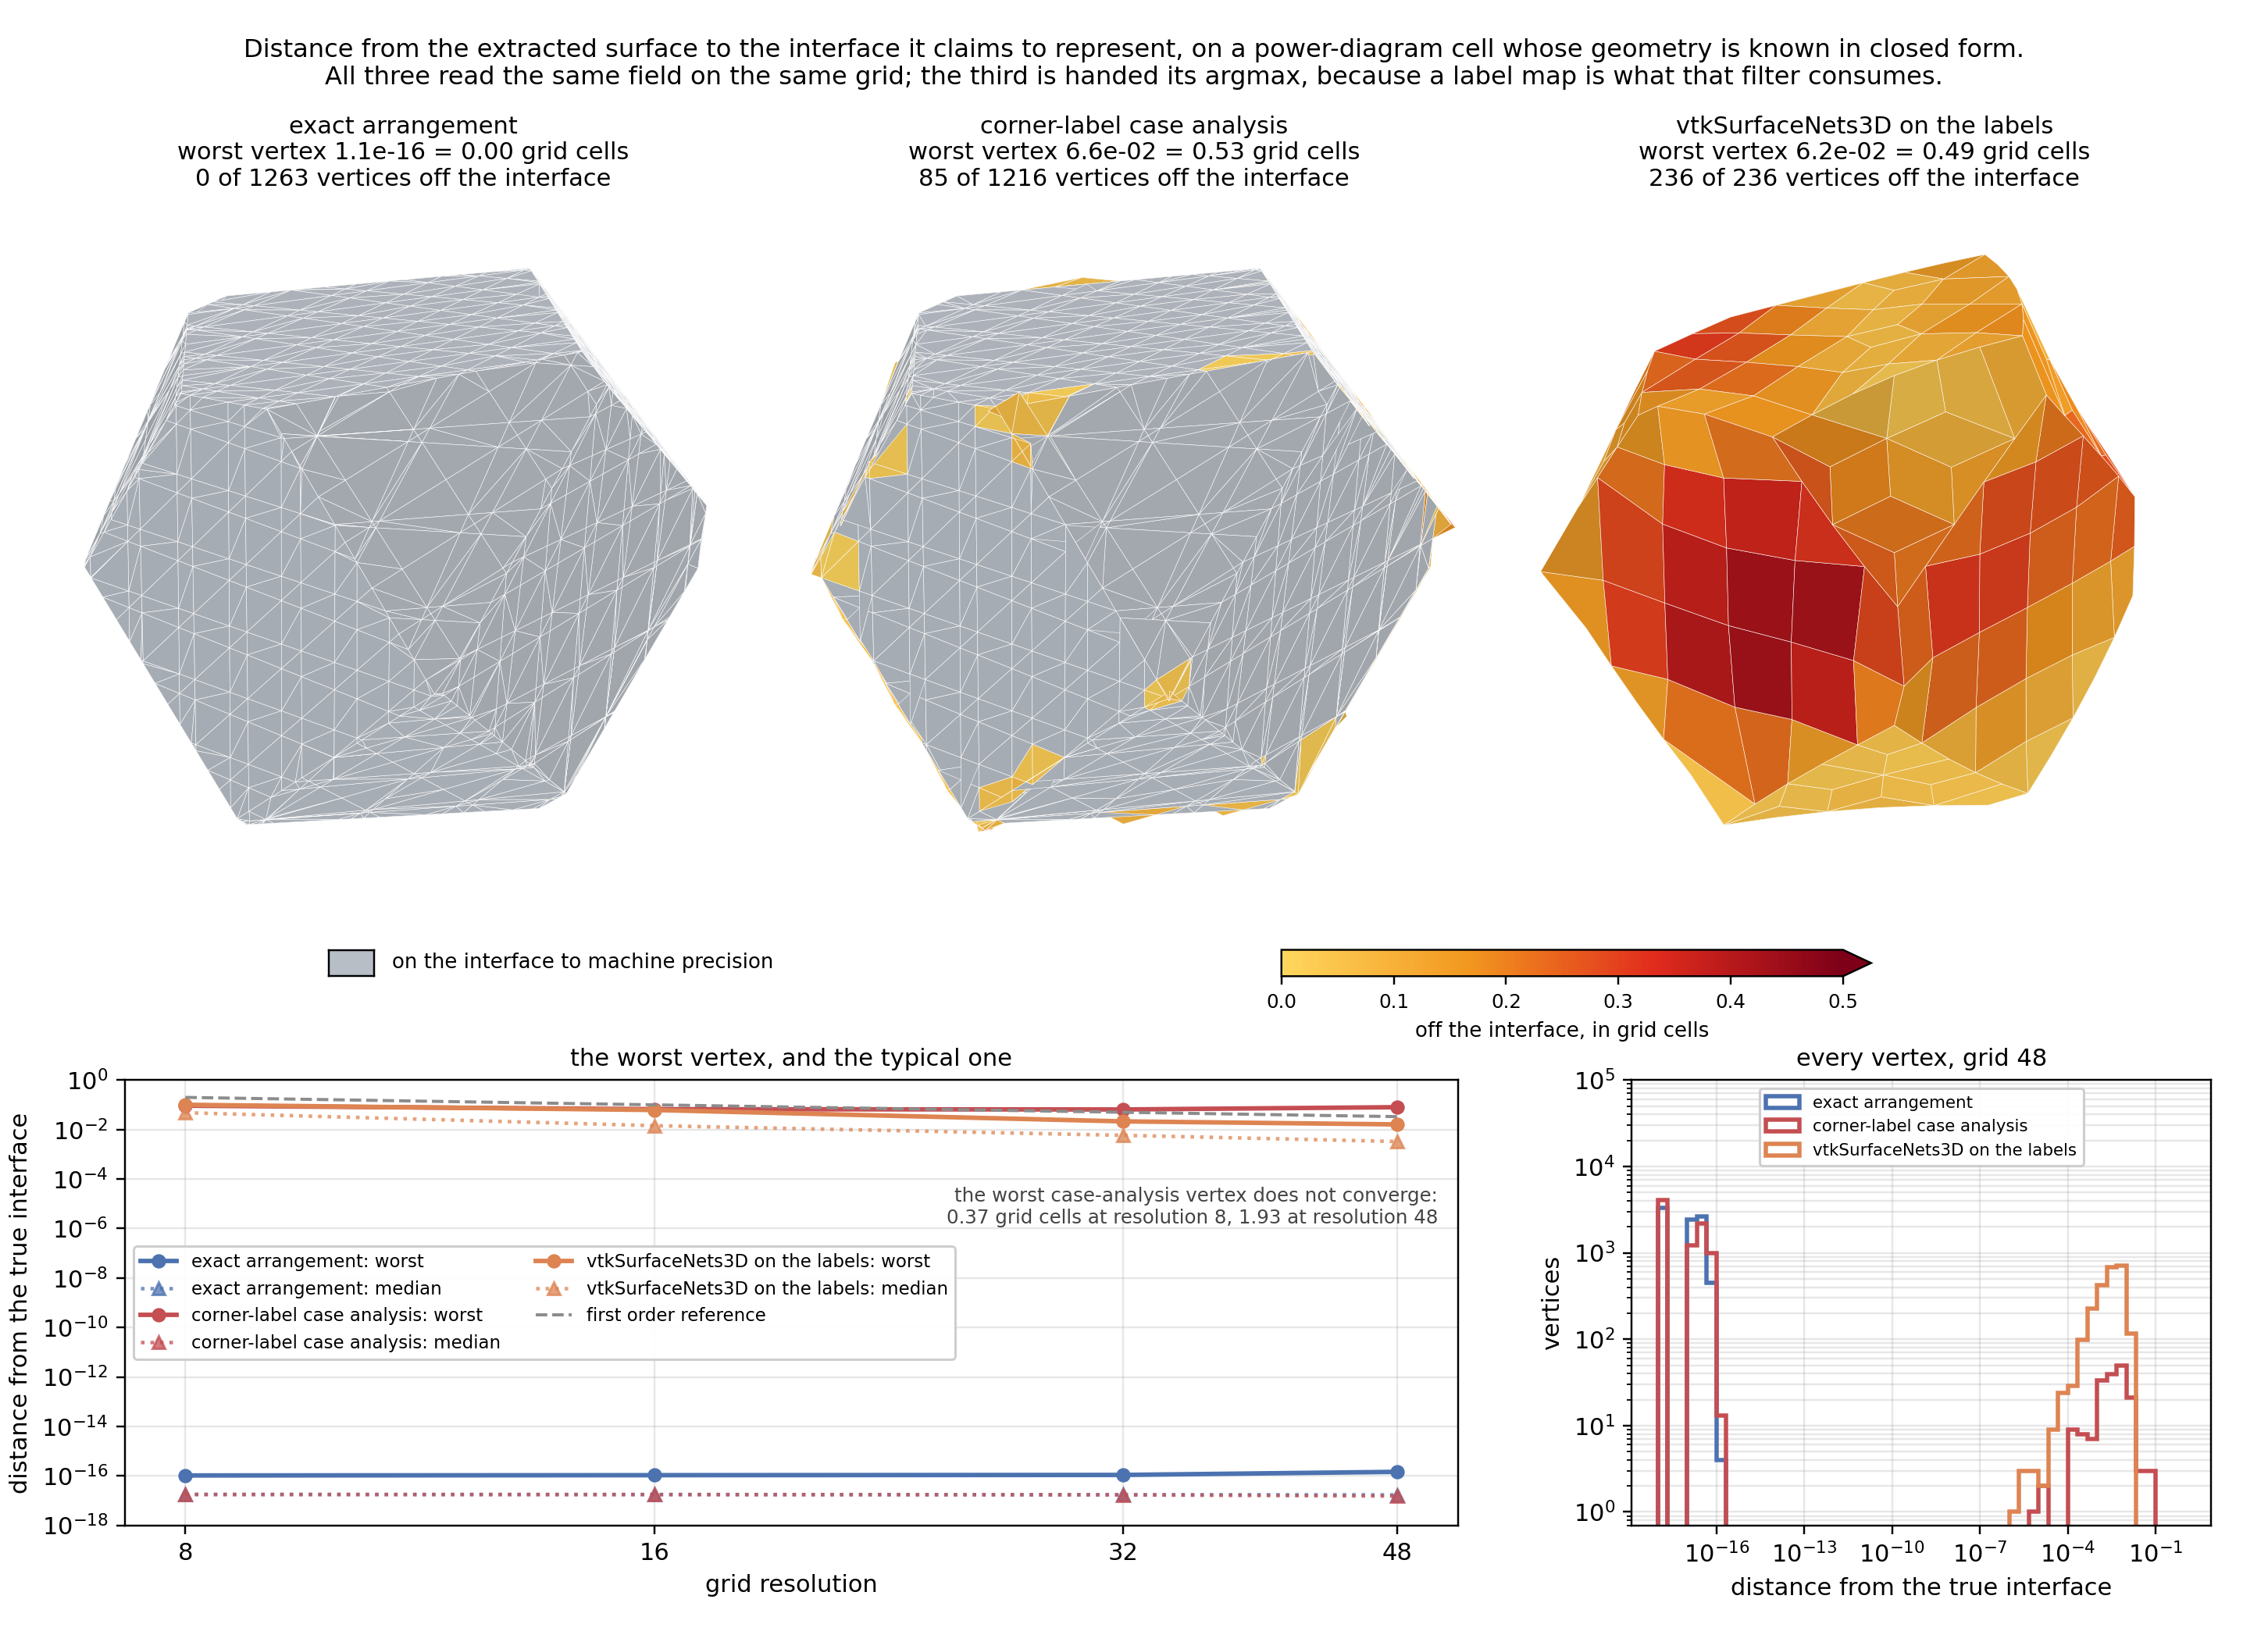
\includegraphics[width=\linewidth]{interface_accuracy.png}
\caption{Distance from each extracted vertex to the interface it claims to lie
on, measured in closed form on the power-diagram cell of Table~\ref{tab:exact}.
Grey faces are on the interface to floating-point precision; coloured ones are
off it, on a scale of grid cells. The arrangement is grey everywhere at every
resolution; case analysis is grey except for a few scars whose worst vertex does not
converge; \texttt{vtkSurfaceNets3D}, given the argmax of the same field because
a label map is what it consumes, is off everywhere and converges at first
order. The arrangement is run with the symbolic perturbation disabled, which
puts its floor at machine precision; enabling it raises the floor to the
perturbation's own magnitude and changes nothing else, as in
Table~\ref{tab:exact}.}
\label{fig:accuracy}
\end{figure}

\section{Curved interfaces}
\label{sec:curved-supp}

On spherical shells the extracted area of a sphere of known radius has relative
error $4.56\times10^{-2}$, $2.01\times10^{-2}$, $1.12\times10^{-2}$,
$5.00\times10^{-3}$ for resolutions $16, 24, 32, 48$, a least-squares fitted
rate of $2.01$ (Figure~\ref{fig:convergence}, right). Second order is what a
$P_1$ interpolant of the logits supports and is the same order as marching cubes
on a smooth two-label field; the point is that adding junctions costs nothing.

\section{Vertices satisfy their defining equations}

As a check independent of the solver, we recompute the interpolant at each
emitted vertex by locating it in the grid and evaluating \eqref{eq:interp}, then
measure the spread among the logits that are supposed to tie. Over five fields at
resolution $14$, the worst spread is $4.4\times10^{-16}$
(power diagram, $2\,499$ vertices), $2.2\times10^{-16}$ (sector fan, $2\,106$),
$6.9\times10^{-17}$ (shells, $3\,402$), $1.1\times10^{-16}$ (neural $K=4$,
$4\,339$) and $1.4\times10^{-16}$ (neural $K=6$, $5\,211$).

\section{Closure and orientability}

Every side of every triangle is examined together with the label pair of its
patch. A side may be used only once if it lies on a triple curve, where three
patches meet along a non-manifold edge, or on $\partial\Omega$, where the
surface is legitimately cut off; every other side must be used exactly twice and
traversed in opposite directions by its two users. Across five fields at
resolutions $12$ and $20$ --- up to $20\,660$ triangles and $31\,880$ sides ---
there are zero unpaired sides, zero inconsistently oriented sides, and zero
patches with too few corners.

Those five fields were chosen for having closed-form answers, so they are not
a fair test of closure on a field nobody arranged. We therefore repeat the
check on forty fields drawn without inspection --- eight seeds each of the
neural field at $K=4$ and $K=6$, and of random power diagrams at $K=4$, $6$
and $9$ --- and none of them produces a single unpaired or inconsistently
oriented side. Closure is not proved, and the propositions of the paper do not
imply it; this is the evidence for it. Figure~\ref{fig:exploded} shows the consequence:
each region is a closed oriented surface, and neighbours share their interface
vertex for vertex. Figure~\ref{fig:arrangement} makes the complementary point
from the outside: the same power diagram extracted at three resolutions is
indistinguishable panel to panel, because on affine logits
(Proposition~\ref{prop:affine}) refinement changes the triangle count and
nothing else.

\begin{figure}[tbp]
\centering
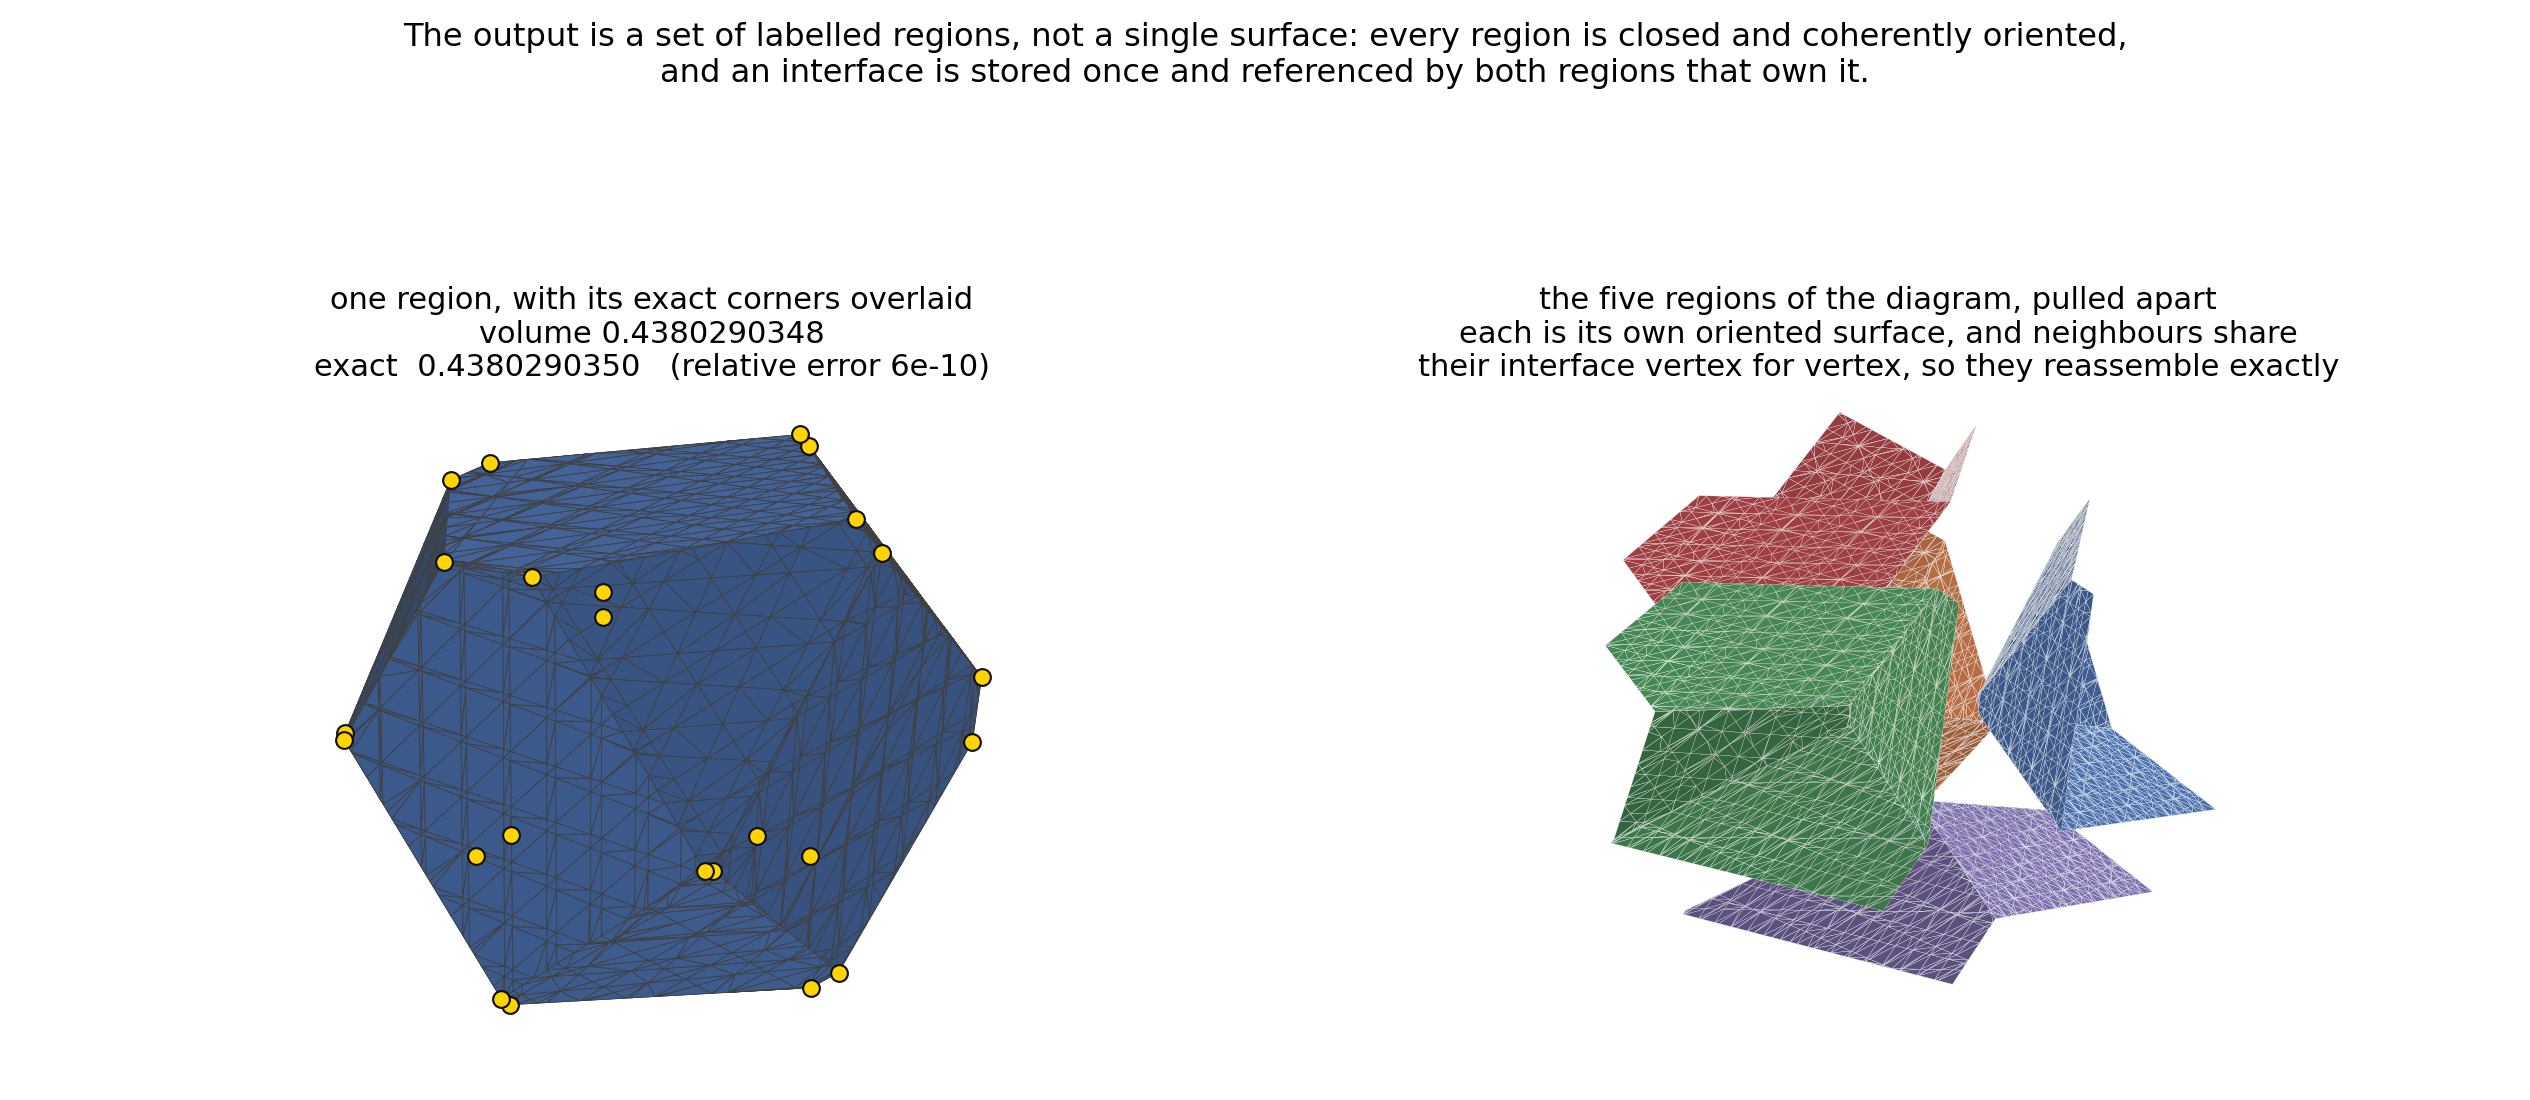
\includegraphics[width=\linewidth]{exploded_regions.png}
\caption{Left: one extracted region with its analytically computed corners
overlaid; the volume agrees with closed form to $6\times10^{-10}$, the residual
being the symbolic perturbation. Right: all five regions of a diagram pulled off
the common centre.}
\label{fig:exploded}
\end{figure}

\section{Features per cell}

Table~\ref{tab:multiplicity} counts the configurations of
Figure~\ref{fig:multifeature} in the test fields. They are common enough that
representing them is not an edge-case concern but a correctness requirement.

\begin{table}[tbp]
\centering
\caption{Cells carrying more than one feature, at resolution $20$. A
one-feature-per-cell case table cannot represent any of these.}
\label{tab:multiplicity}
\begin{tabular}{@{}lrr@{}}
\toprule
field & edges with $\ge 2$ crossings & faces with $\ge 2$ triple points \\
\midrule
power diagram ($K=5$)  & 46 & 3 \\
sector fan ($K=4$)     & 21 & 0 \\
spherical shells ($K=4$) & 0 & 0 \\
neural field ($K=4$)   & 67 & 5 \\
neural field ($K=6$)   & 71 & 0 \\
\midrule
total & 205 & 8 \\
\bottomrule
\end{tabular}
\end{table}

\section{Gradients}

We compare reverse-mode autograd against central finite differences of a
permutation-invariant loss on the extracted vertices. The loss must not depend
on vertex order, because perturbing a parameter can reorder the output without
moving the surface; probes at which the vertex count changes are genuine
topology changes, where a difference quotient is meaningless, and are skipped
and counted. Worst relative errors are $1.2\times10^{-8}$ for a power diagram
differentiated with respect to all sites and weights ($20$ probes),
$1.9\times10^{-8}$ for shells with respect to radii, $1.2\times10^{-10}$ for a
sector fan with respect to its centre, and $7.6\times10^{-6}$ for a neural field
with respect to its entire weight vector ($79$ probes, $2$ skipped).

\section{Plateau's angle}

On a symmetric sector fan the dihedral angles along triple curves are computed
from field gradients, which is the correct measurement: the $k|l$ patch is the
level set of $f_k-f_l$ and its normal at the curve is exactly
$\nabla(f_k-f_l)$ there, whereas measuring from mesh geometry would carry an
$O(h)$ curvature bias. Over $155$ segments the worst deviation from $120^\circ$
is $1.4\times10^{-14}$ degrees (Figure~\ref{fig:plateau}), consistent with
Proposition~\ref{prop:plateau}.

\begin{figure}[tbp]
\centering
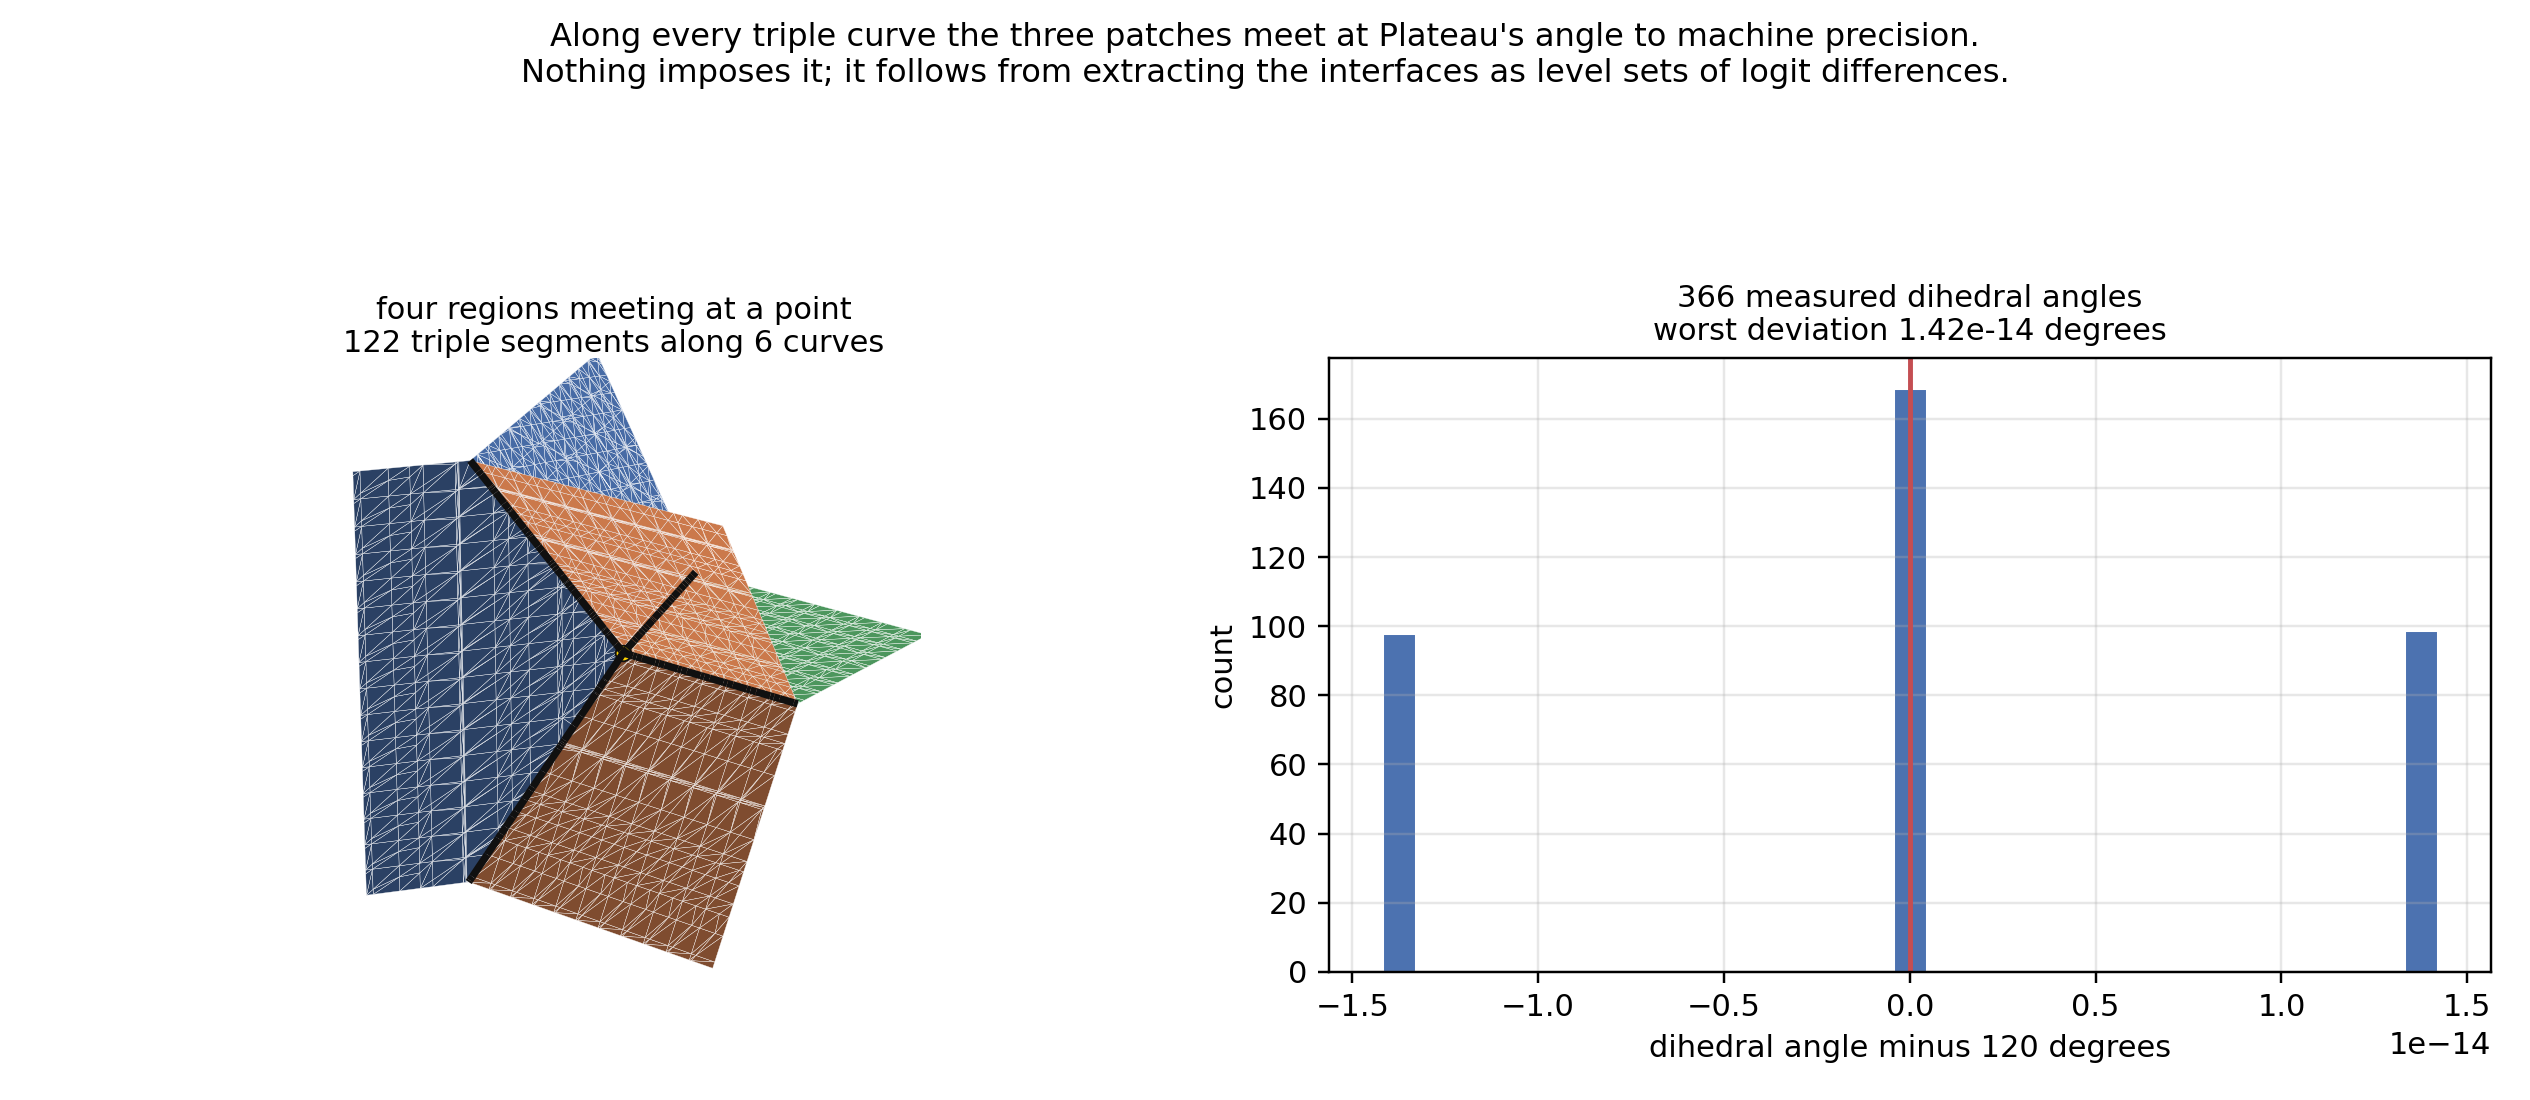
\includegraphics[width=0.86\textwidth]{triple_curves_120.png}
\caption{Dihedral angles along the triple curves of a symmetric sector fan.
Plateau's condition is satisfied identically rather than approximately
(Proposition~\ref{prop:plateau}).}
\label{fig:plateau}
\end{figure}

\section{The 2D instantiation and optimisation through the extractor}
\label{sec:2d-supp}

The same construction in 2D --- crossings on edges of a triangular grid,
junctions inside triangles --- gives a self-contained extractor which we use to
study optimisation, and which passes $24$ checks of its own. Triple point
positions match the closed-form Voronoi circumcentre to $8.4\times10^{-17}$, and
the \emph{Jacobian} of a junction with respect to the sites matches the
analytic derivative of the circumcentre to $2.9\times10^{-16}$ --- a stronger
statement than a finite-difference agreement, since it compares against a
formula. Interface vertices lie on exact circles to $2.2\times10^{-16}$, and
polyline midpoint error converges at fitted rate $1.93$.

Two downstream studies exercise the gradients.
\emph{Target matching}: a randomly initialised neural field with $K=3$ is
optimised so that its extracted partition matches a target partition, reducing
the loss from $0.689$ to $0.0077$ ($98.9\%$) in $260$ steps
(Figure~\ref{fig:target}).
\emph{Minimal interfaces}: we minimise total interface length under equal-area
constraints on a disk, where the analytic minimiser is the three-fold
$120^\circ$ configuration of total length $3R$. Optimising a power-diagram field
reaches length $2.4000$ against the exact $2.40$ and angles
$119.6^\circ, 120.1^\circ, 120.3^\circ$ from an initial
$113.9^\circ, 120.8^\circ, 125.3^\circ$ (Figure~\ref{fig:plateau2d}). The same
objective on a neural field improves the length but converges to
$114.5^\circ, 114.6^\circ, 130.9^\circ$; the extractor is identical in both
runs, so this reflects the optimisation landscape of the over-parameterised
representation rather than the extraction, and we report it as a negative result
rather than tuning it away.

\begin{figure}[tbp]
\centering
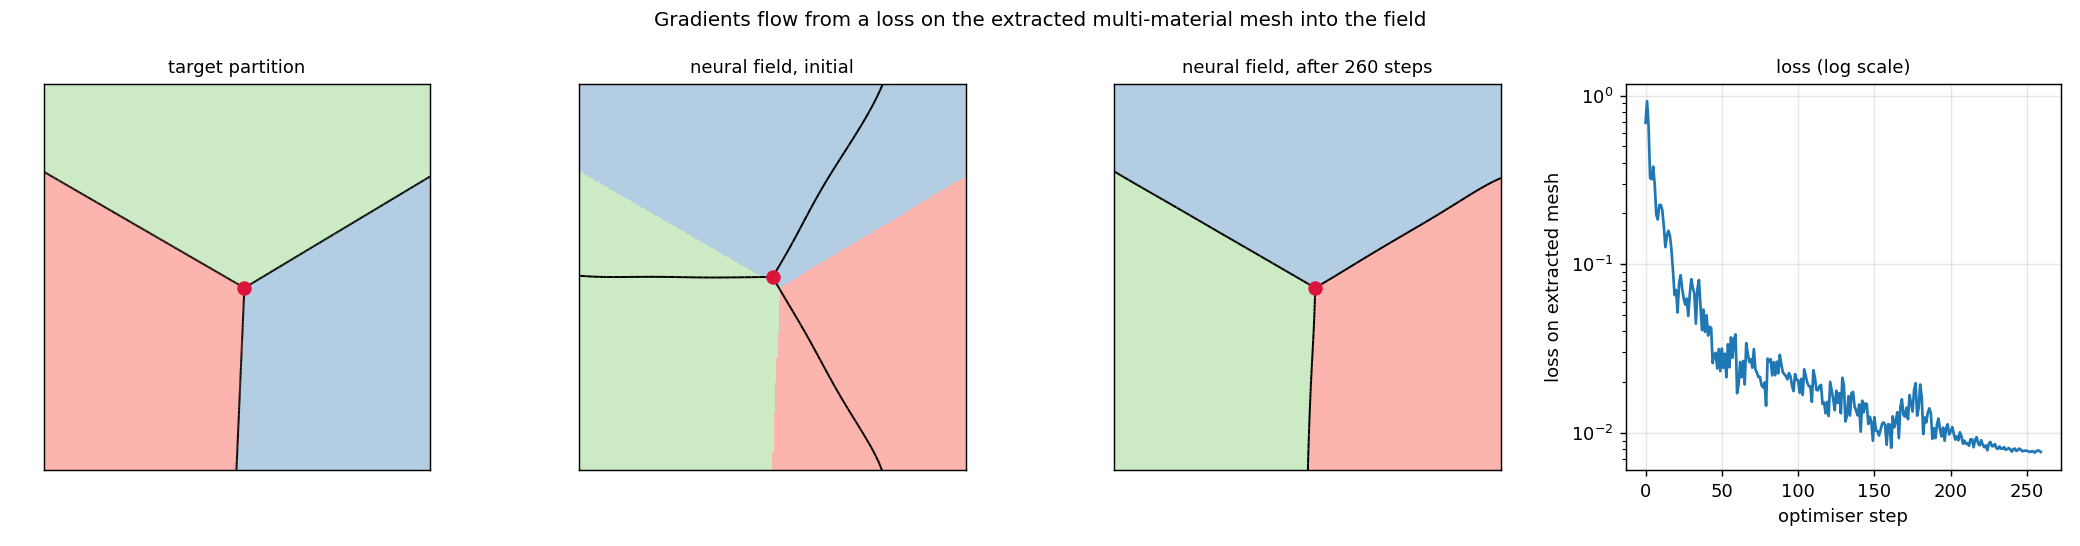
\includegraphics[width=\linewidth]{target_matching.png}
\caption{Target matching in 2D: a randomly initialised $K=3$ neural field
(left) optimised until its extracted partition matches the target (right),
which takes the loss from $0.689$ to $0.0077$ in $260$ steps. Gradients from a
loss written on the extracted mesh flow back into the field parameters.}
\label{fig:target}
\end{figure}

\begin{figure}[tbp]
\centering
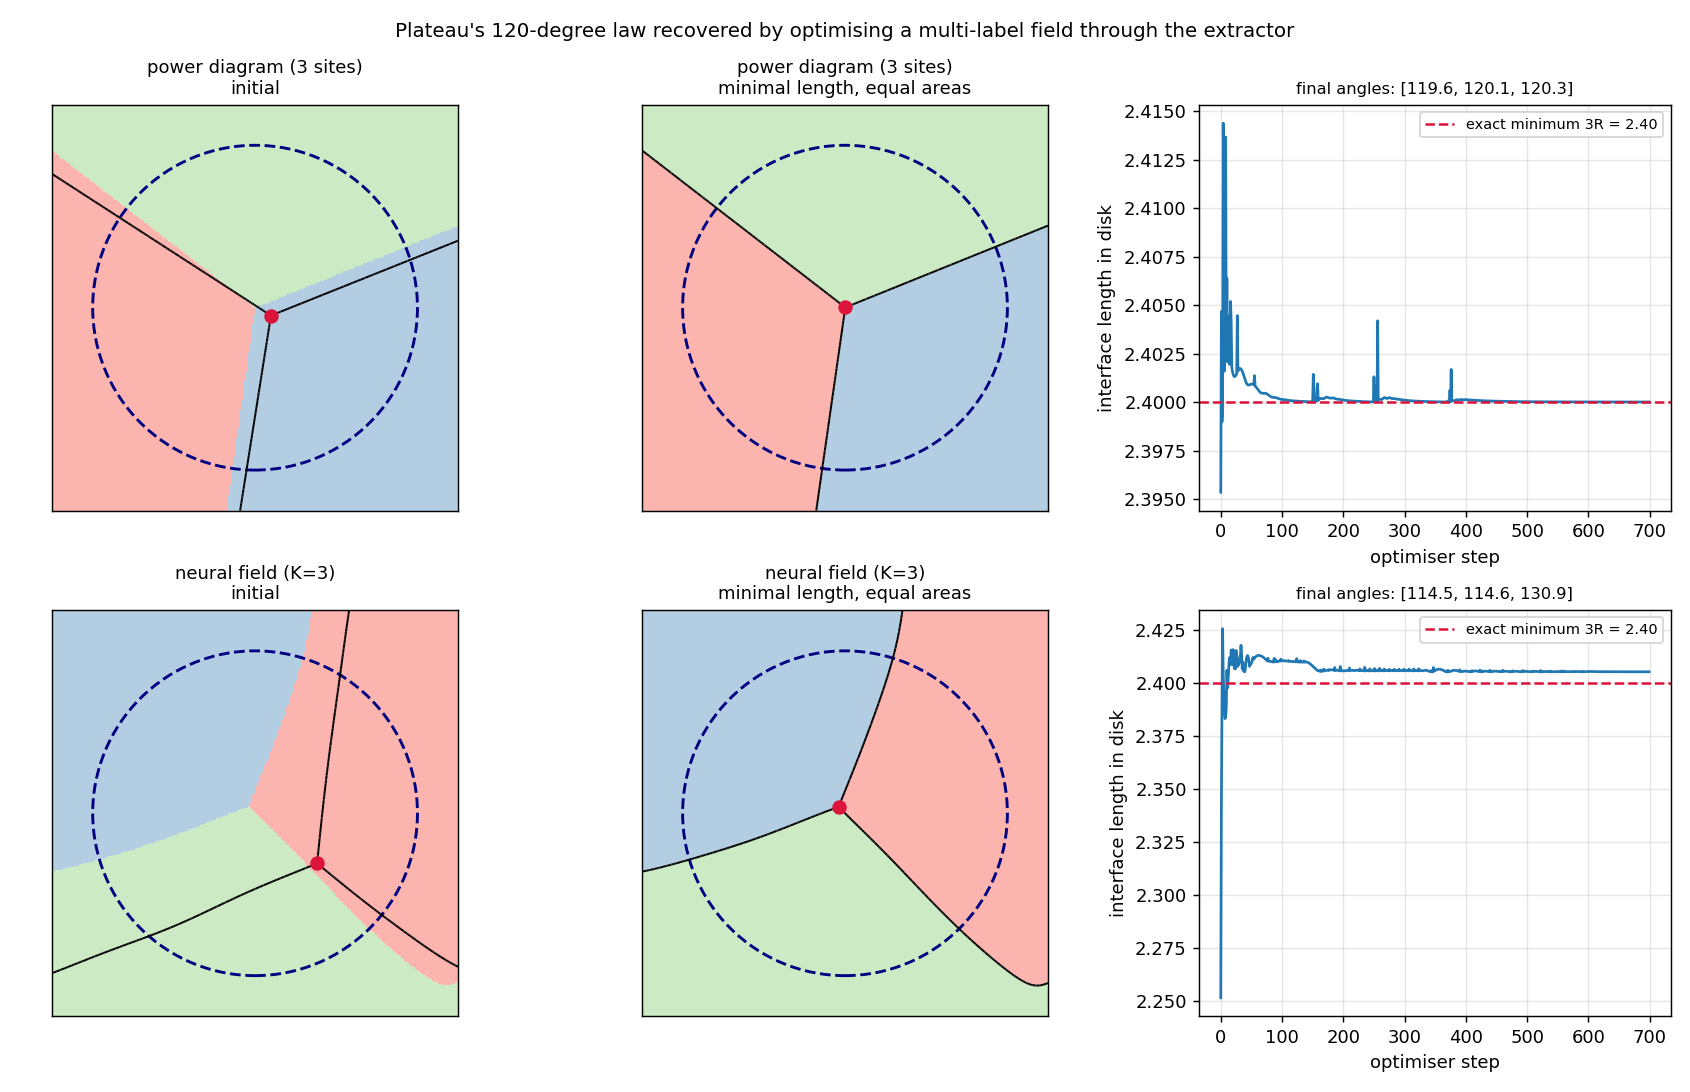
\includegraphics[width=0.9\textwidth]{plateau_disk.png}
\caption{Minimising interface length under equal-area constraints recovers the
analytic $120^\circ$ minimiser for a power-diagram field (top). The same
objective on a neural field (bottom) improves the length but stalls short of the
minimiser.}
\label{fig:plateau2d}
\end{figure}

\begin{figure}[tbp]
\centering
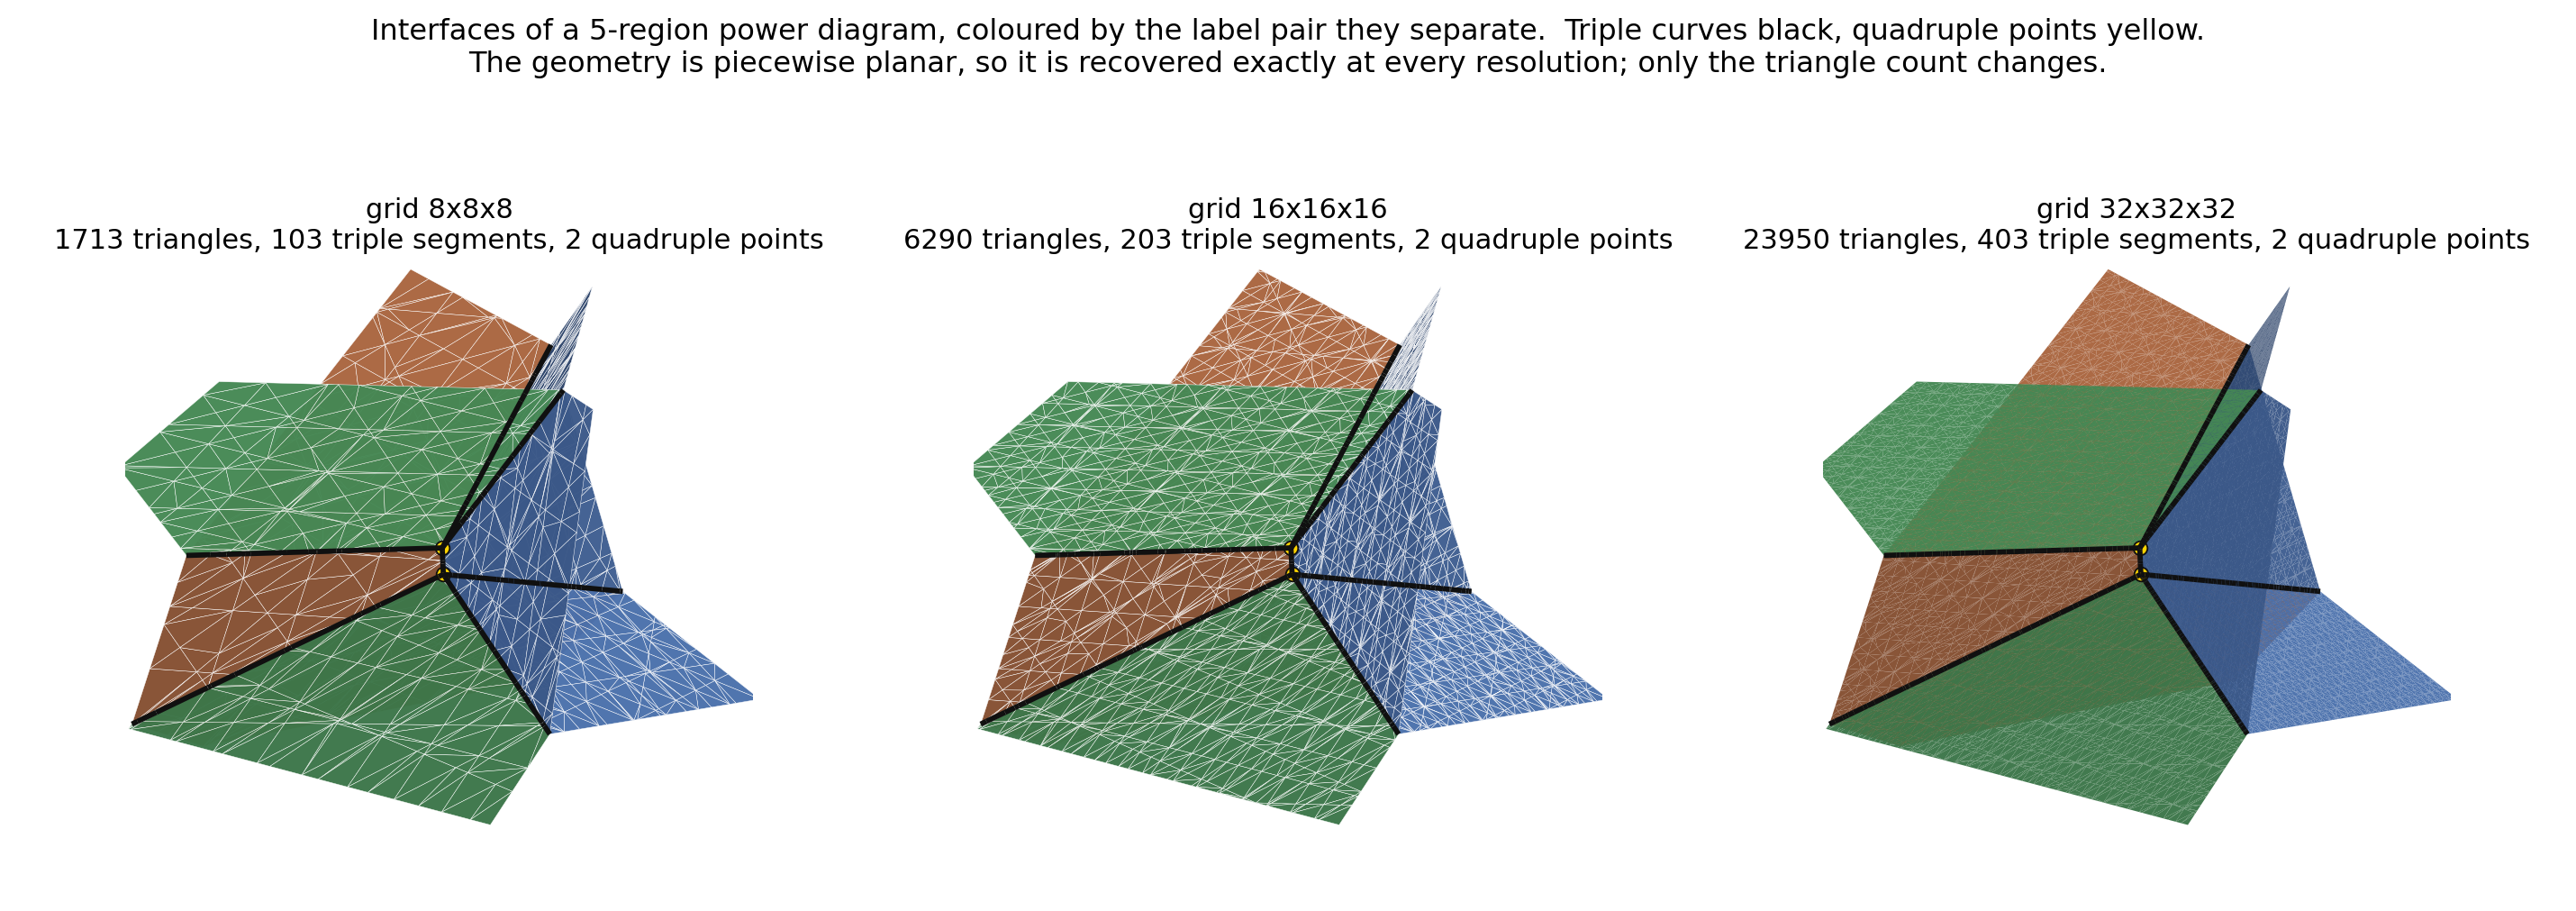
\includegraphics[width=\linewidth]{arrangement_3d.png}
\caption{A five-region power diagram at three resolutions. The panels being
indistinguishable is the content: by Proposition~\ref{prop:affine} the geometry
is recovered exactly at each, and only the triangle count changes.}
\label{fig:arrangement}
\end{figure}


\section{Contact between solid objects, in full}
\label{sec:contact-supp}

Section~\ref{sec:contact} reports the accuracy of the contact set in summary.
The closed forms it is judged against come from two balls of radius $r$ whose
centres are $s$ apart: on the bisector plane both interior logits equal $r^2 -
s^2/4 - y^2 - z^2$, so the patch is a disk of radius $a=\sqrt{r^2-s^2/4}$ and
\[
  A(s) = \pi\!\left(r^2 - \tfrac{s^2}{4}\right),\quad
  \frac{\mathrm{d}A}{\mathrm{d}s} = -\frac{\pi s}{2},\quad
  L(s) = 2\pi\sqrt{r^2 - \tfrac{s^2}{4}},
\]
for $s<2r$ and zero beyond. Table~\ref{tab:contact} walks $s$ across that
range. The errors track $a/h$, the patch radius in cells, rather than the
separation: a patch interior is reproduced exactly because $f_i-f_j$ is affine
and its $P_1$ interpolant is itself, so the whole error lies in where the
boundary falls, and a disk a few cells across cannot place one. The derivative
column is reverse-mode autograd through the extraction, converted to
$\mathrm{d}/\mathrm{d}s$ by the chain rule. Agreeing with the closed form
establishes that the geometry is right, not that the gradient is attached to
what the code computed; the central-difference check at $s=0.70$ does that,
matching to $1.5\times10^{-10}$ relative on the patch area and
$1.2\times10^{-10}$ on the rim length.

The three-object configuration places three balls of radius $r$ with centres on
a circle of radius $R$. All three interior logits tie on the axis through that
circle's centre, and the background joins the tie where additionally $f_0=0$,
which puts quadruple points at height $\pm\sqrt{r^2-R^2}$ either side of the
plane of centres, with the three contact patches meeting along the segment
between them. At resolution $48$ the extractor returns exactly two such points,
at $-0.355679$ and $+0.355835$ against the exact $\pm0.357071$, and a triple
curve of length $0.711514$ against the exact $0.714143$. The three patches,
equal by symmetry, agree with each other to $8.5\times10^{-4}$ despite a grid
sharing none of that symmetry. Of the complex's $39\,946$ triangles, $6\,236$
carry an object--object label pair, and each of those is one triangle belonging
to two objects rather than two triangles that have to be reconciled.

\begin{table*}[tbp]
\centering
\caption{Two objects walked apart, at resolution $48$ with $r=0.45$, cell size
$h=0.0417$. Closed forms as above; $a/h$ is the exact patch radius in cells.
The derivative column is reverse-mode autograd through the extraction, not a
difference quotient. At and beyond onset the patch does not exist and every
entry is identically zero.}
\label{tab:contact}
\begin{tabular}{@{}rrrrrrrr@{}}
\toprule
& & \multicolumn{2}{c}{patch area $A$} & \multicolumn{2}{c}{$\mathrm{d}A/\mathrm{d}s$} & \multicolumn{2}{c}{rim length $L$} \\
\cmidrule(lr){3-4}\cmidrule(lr){5-6}\cmidrule(l){7-8}
$s/2r$ & $a/h$ & value & rel.\ err & value & rel.\ err & value & rel.\ err \\
\midrule
$0.40$ & $9.9$ & $0.531388$ & $5.6\!\times\!10^{-3}$ & $-0.56266$ & $5.0\!\times\!10^{-3}$ & $2.58524$ & $2.4\!\times\!10^{-3}$ \\
$0.60$ & $8.6$ & $0.404279$ & $7.1\!\times\!10^{-3}$ & $-0.84663$ & $1.9\!\times\!10^{-3}$ & $2.25530$ & $2.9\!\times\!10^{-3}$ \\
$0.75$ & $7.1$ & $0.275223$ & $1.1\!\times\!10^{-2}$ & $-1.05793$ & $2.2\!\times\!10^{-3}$ & $1.86136$ & $4.7\!\times\!10^{-3}$ \\
$0.85$ & $5.7$ & $0.173689$ & $1.6\!\times\!10^{-2}$ & $-1.19312$ & $7.1\!\times\!10^{-3}$ & $1.47955$ & $6.6\!\times\!10^{-3}$ \\
$0.92$ & $4.2$ & $0.094584$ & $3.2\!\times\!10^{-2}$ & $-1.30194$ & $1.0\!\times\!10^{-3}$ & $1.09295$ & $1.4\!\times\!10^{-2}$ \\
$0.96$ & $3.0$ & $0.046816$ & $6.1\!\times\!10^{-2}$ & $-1.31257$ & $3.3\!\times\!10^{-2}$ & $0.77149$ & $2.6\!\times\!10^{-2}$ \\
$0.99$ & $1.5$ & $0.009581$ & $2.4\!\times\!10^{-1}$ & $-1.61520$ & $1.5\!\times\!10^{-1}$ & $0.35666$ & $1.1\!\times\!10^{-1}$ \\
$1.00$ & $0$   & $0$        & ---                    & $0$        & ---                    & $0$       & --- \\
$1.02$ & ---   & $0$        & ---                    & $0$        & ---                    & $0$       & --- \\
\bottomrule
\end{tabular}
\end{table*}

\section{Clinical field: interface accuracy}
\label{sec:realdata-supp}

Section~\ref{sec:realdata} summarises the median and tail distances;
Figure~\ref{fig:realdataacc} is the per-vertex map behind them. Against the
trilinear interpolant on the segment-to-segment walls, our vertices sit a
median of $0.0095$ voxels from it and SurfaceNets' $0.090$; at the $90$th
percentile the figures are $0.074$ and $0.231$ voxels. Measuring our vertices
against the $P_1$ interpolant they are built on would be circular, which is why
the comparison is made against a third interpolant neither method is defined
on.

\begin{figure}[tbp]
\centering
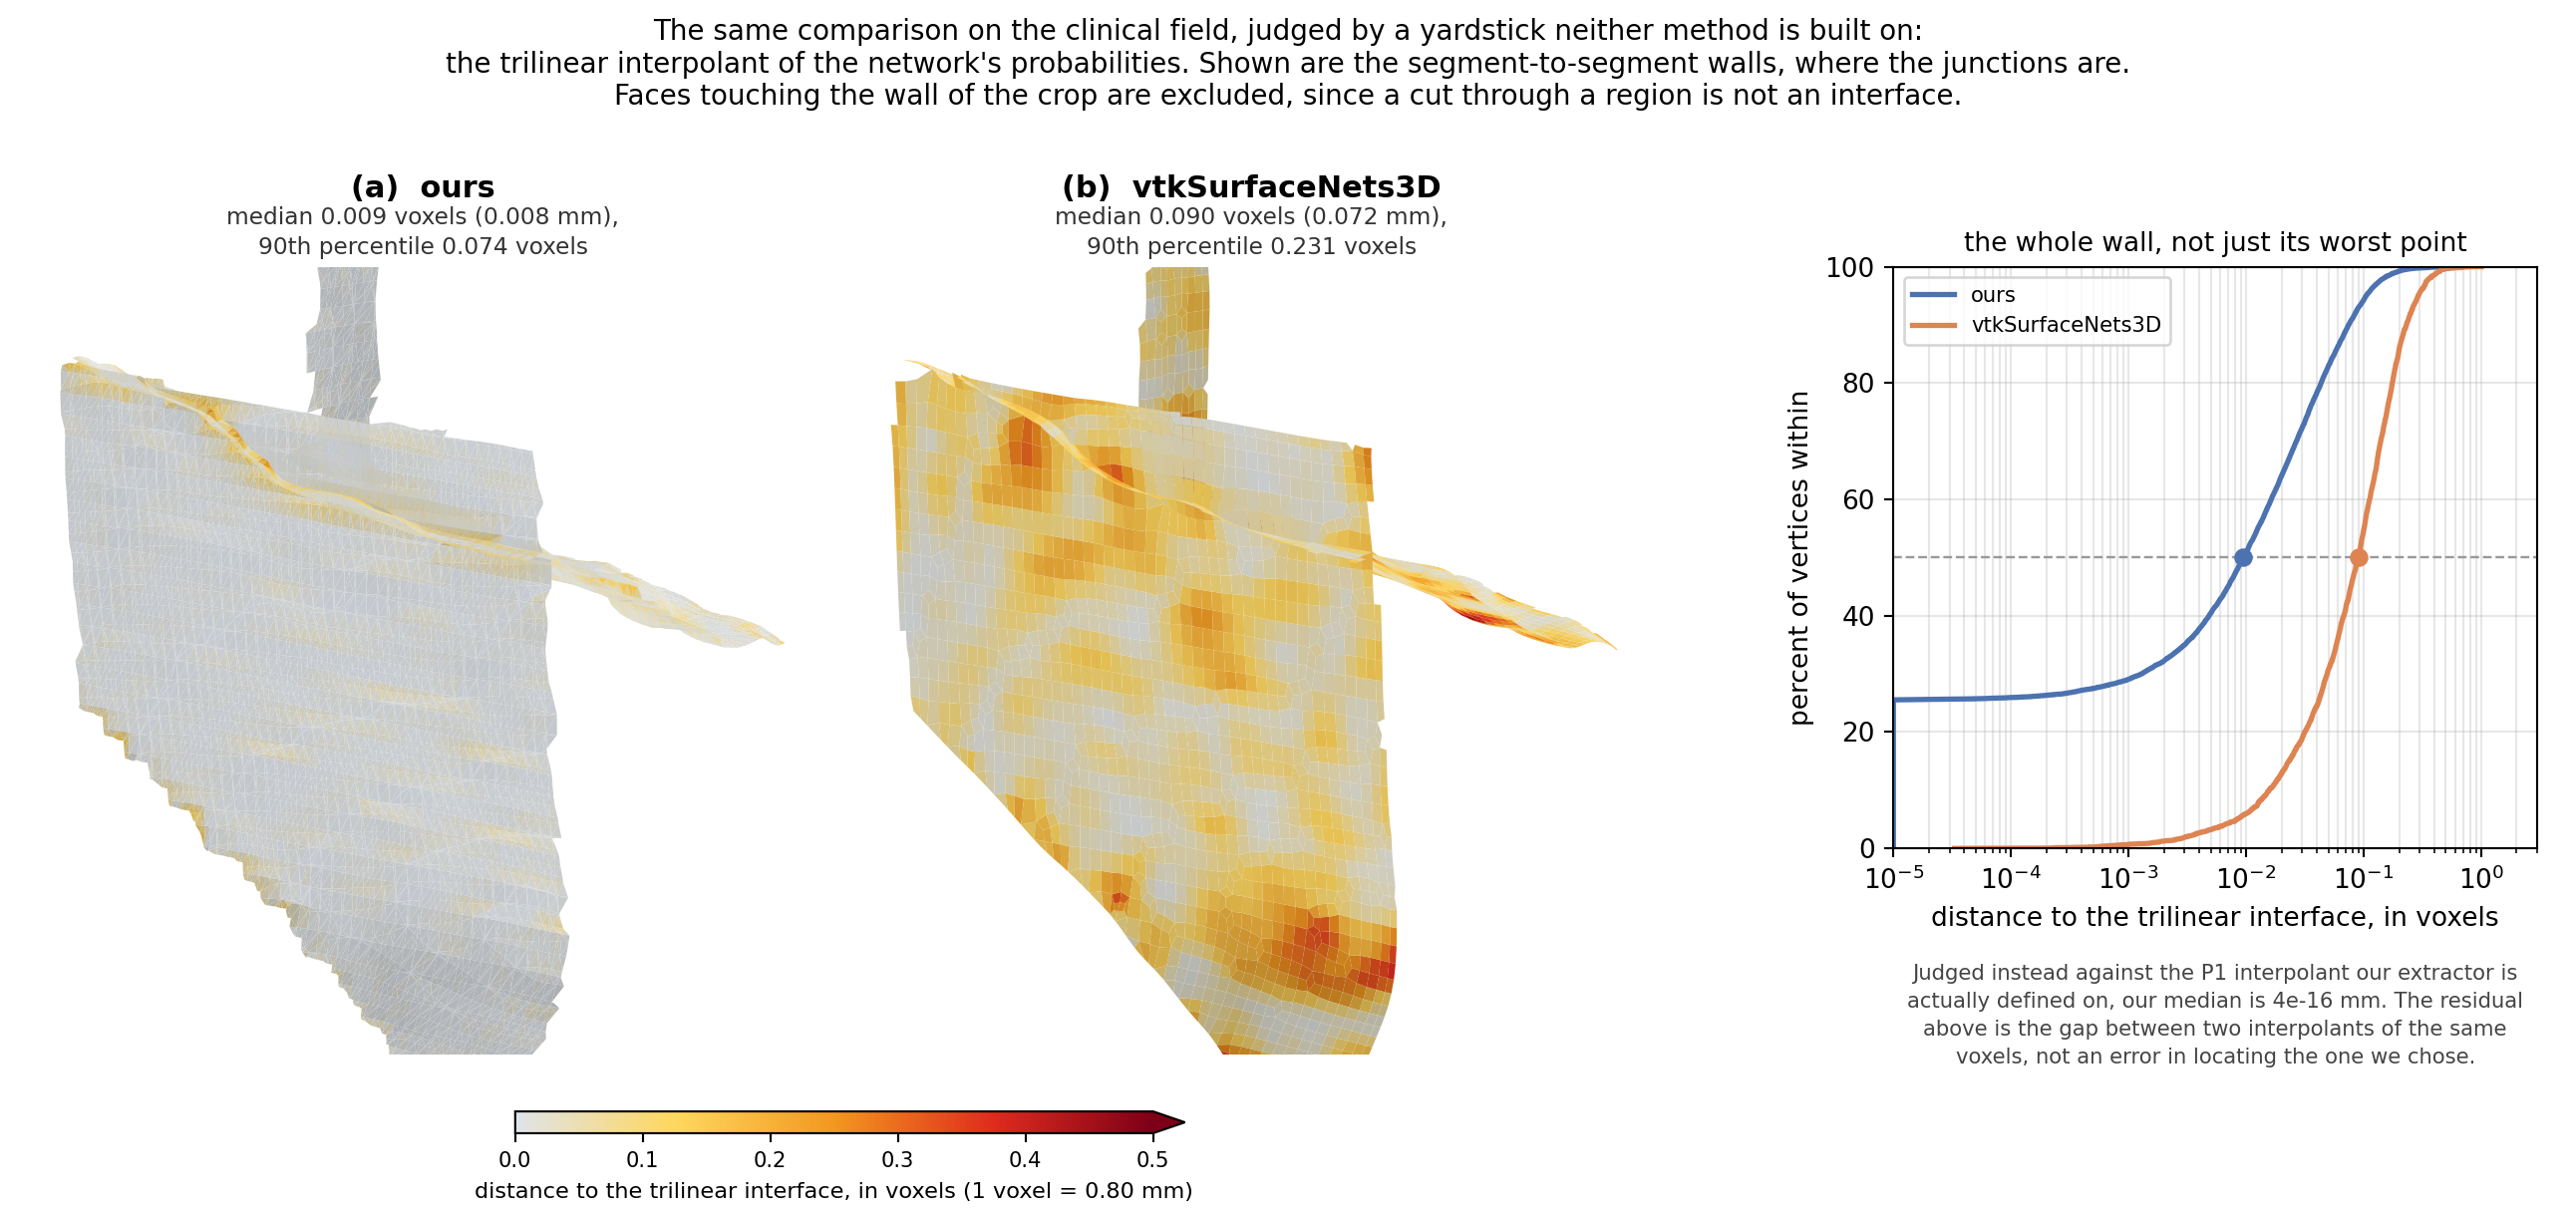
\includegraphics[width=\linewidth]{realdata_accuracy.png}
\caption{The clinical field judged by an interpolant neither method is defined
on: the trilinear one, on the segment-to-segment walls of the liver-segment
window of Section~\ref{sec:realdata} of the paper. Pale is on the interface; colour is off it,
in voxels. The liver's outer shell is omitted because it would hide the
junctions, and faces meeting the wall of the
crop are dropped from both the picture and the numbers, a cut through a region
not being an interface. Since the trilinear field is not affine the measure is
a first-order distance, which is enough to separate two meshes a tenth of a
voxel apart.}
\label{fig:realdataacc}
\end{figure}

\section{Agreement with the exact baseline, in full}
\label{sec:headtohead-supp}

Section~\ref{sec:headtohead} states the result; this is the case list behind
it and the detail of the one input on which the two implementations differ.

Their tool normally generates its own grid, so ours is passed through its
\texttt{tetMeshFile} input and both read the same tetrahedra. Its loader
evaluates analytic primitives at the vertices, which covers the sphere and
plane cases; for fields with no closed form we add twenty-nine lines to that
loader so it can also read per-vertex values. The addition fills the same
matrix column every existing branch fills and changes no line of the
arrangement code. The control row of Table~\ref{tab:headtohead} tests exactly
that, sending a field their loader can evaluate analytically down the
per-vertex path instead and requiring the same answer. Nothing else is
modified, and our symbolic perturbation is off, since a displacement they do
not apply would guarantee a mismatch at precisely the configurations worth
comparing. The container recipe that builds their code, the loader patch and
the harness that drives both are released alongside ours.

\begin{table}[tbp]
\centering
\small
\caption{Our extractor against the reference implementation of Du et
al.~\cite{du2022} on identical tetrahedra. Vertices, polygons and patches are
their \texttt{num\_MI\_verts}, \texttt{num\_MI\_faces} and
\texttt{num\_patches}; a single entry means the two produced the same value.
A patch here is theirs: a connected union of same-pair polygons, which is why
the clinical row reads $16$ where Section~\ref{sec:realdata} counts $11$
distinct labelled interfaces on the same window.
The last column is the symmetric nearest-neighbour distance between the two
vertex sets. The final row leaves the clinical field's exact coincidences in
place, which is the one input on which the two differ; entries are
theirs/ours.}
\label{tab:headtohead}
\begin{tabular}{@{}lrrrrrr@{}}
\toprule
field & $K$ & tets & vertices & polygons & patches & vertex gap \\
\midrule
\multicolumn{7}{@{}l}{\emph{their primitives, evaluated analytically at both ends}} \\
\quad their 18-sphere example & $18$ & $55\,566$ & $12\,201$ & $17\,885$ & $70$ & $3.3\!\times\!10^{-16}$ \\
\quad 8 spheres               & $8$  & $82\,944$ & $8\,581$  & $12\,629$ & $16$ & $3.1\!\times\!10^{-16}$ \\
\quad 5 planes                & $5$  & $82\,944$ & $5\,798$  & $8\,435$  & $9$  & $3.2\!\times\!10^{-16}$ \\
\quad 12 planes               & $12$ & $48\,000$ & $6\,775$  & $9\,892$  & $27$ & $3.5\!\times\!10^{-16}$ \\
\addlinespace
\multicolumn{7}{@{}l}{\emph{delivered to them as per-vertex values}} \\
\quad 5 planes (control)      & $5$  & $82\,944$ & $5\,798$  & $8\,435$  & $9$  & $3.2\!\times\!10^{-16}$ \\
\quad power diagram           & $5$  & $82\,944$ & $6\,953$  & $10\,382$ & $9$  & $4.6\!\times\!10^{-16}$ \\
\quad neural field            & $6$  & $82\,944$ & $15\,051$ & $21\,916$ & $10$ & $3.7\!\times\!10^{-16}$ \\
\quad clinical liver, generic & $9$  & $663\,552$& $34\,762$ & $51\,617$ & $16$ & $1.1\!\times\!10^{-14}$ \\
\addlinespace
\multicolumn{7}{@{}l}{\emph{with exact coincidences left in the input}} \\
\quad clinical liver, as given& $9$  & $663\,552$& $34\,707/34\,644$ & $51\,565/51\,522$ & $16$ & --- \\
\bottomrule
\end{tabular}
\end{table}

\paragraph*{The one disagreement, and what it is.} The clinical field as
acquired is the single input on which the two differ, for the reason
Section~\ref{sec:degeneracy} anticipates. Ten of its $117\,649$ nodes carry an
exact argmax tie and its smallest nonzero margin is $2.2\times10^{-16}$, one
unit in the last place --- so no displacement is both small enough to leave the
genuine gaps alone and large enough to be representable. There the arrangement
is not unique and the two break the tie differently: theirs symbolic, ours by
displacement, giving $34\,644$ vertices against their $34\,707$, or $34\,764$
with the perturbation on at $10^{-9}$. The discrepancy stays below $0.2\%$ and
remains local to the coincidences: the patch count, the labels and the set of
interfaces present agree throughout, and with the perturbation on every vertex
of theirs lies within $1.7\times10^{-9}$ of one of ours. That gap is the
perturbation itself, and it scales with it: $1.7\times10^{-11}$,
$1.7\times10^{-10}$ and $1.7\times10^{-9}$ at $\varepsilon = 10^{-11}$,
$10^{-10}$ and $10^{-9}$. That is the $O(\delta)$ behaviour measured in
Section~\ref{sec:degentest-supp} of this document, now seen against an independent implementation rather
than against closed form. Displacing the data once, before either extractor
reads it, so that the coincidences are gone from the input both are given,
restores exact agreement. The difference is therefore one of tie-breaking where
the answer is not unique, not of construction.

\paragraph*{Cost.} Their arrangement takes $16$--$178$\,ms across these cases
and ours $102$\,ms--$1.2$\,s, a factor of two to nine depending on the case,
single-threaded, our Python against their optimised C++ with a precomputed
lookup table. These are wall-clock figures from one machine and move by some
tens of percent between runs; the transcript they are read from is released
with the code. Neither side was tuned for the comparison, and the ordering is
unlikely to reverse.


\section{FlexiCubes, in full}
\label{sec:flexicubes-supp}

Tables for Section~\ref{sec:flexicubes}. FlexiCubes runs in float32 throughout,
because its working buffers are allocated at the ambient default dtype while
its default weight tensors are single precision; all of ours runs in
float64. Each method is therefore in the precision it was written for.

\paragraph*{Extraction from a fixed field.} Table~\ref{tab:fcaccuracy} reports
the same analytic field extracted with both, at matched grids --- identical node
and cell counts, identical sample locations --- with no optimisation and their
weights at their defaults, which is how the method would be used on a field
that is already known. At defaults their extractor is dual marching cubes, and
we say so because their own position is that the learned weights are where
their method's advantage lies; the weights cannot be learned without something
to learn against, and there is no loss here.

Two error columns are given, and the distinction is not cosmetic. Scoring the
extracted vertices measures our interpolation error and little else, since our
vertices are by construction the zeros of the $P_1$ interpolant along tetrahedron
edges; a dual vertex is a weighted average of its cell's crossings and is not
intended to lie on the surface at all, even where the mesh approximates it
well. Sampling a fixed budget of points uniformly by area asks the same
question of both, and is what Section~\ref{sec:flexicubes} quotes. On that
measure we are the more accurate on all three statistics at every resolution,
by two to $2.3$ in the root mean square and $1.2$ to $1.7$ at worst, and we
spend about three times as many triangles for it. On the vertex measure the
mean gap widens in our favour and the worst case on the torus reverses to
theirs --- which is the artefact, not the finding. Both converge at second
order on area.

\begin{table}[tbp]
\centering
\caption{Extraction accuracy at $K=2$ from a fixed field. Error is distance to
the analytic surface in grid cells, over points drawn uniformly by area
($d/h$) and over the extracted vertices ($d_v/h$). The sampled columns are the
comparable ones; see the text.}
\label{tab:fcaccuracy}
\small
\begin{tabular}{@{}llrrrrrr@{}}
\toprule
& res & triangles & area error & max $d/h$ & rms $d/h$ & max $d_v/h$ & rms $d_v/h$ \\
\midrule
\multicolumn{8}{@{}l}{\emph{sphere}} \\
ours       & 16 & $2\,592$  & $1.05\!\times\!10^{-2}$ & $0.070$ & $0.036$ & $0.061$ & $0.021$ \\
FlexiCubes & 16 & $828$     & $2.73\!\times\!10^{-2}$ & $0.121$ & $0.081$ & $0.070$ & $0.051$ \\
ours       & 32 & $10\,968$ & $2.62\!\times\!10^{-3}$ & $0.036$ & $0.018$ & $0.034$ & $0.010$ \\
FlexiCubes & 32 & $3\,660$  & $6.23\!\times\!10^{-3}$ & $0.060$ & $0.040$ & $0.035$ & $0.025$ \\
ours       & 48 & $24\,912$ & $1.16\!\times\!10^{-3}$ & $0.025$ & $0.012$ & $0.025$ & $0.007$ \\
FlexiCubes & 48 & $8\,364$  & $2.77\!\times\!10^{-3}$ & $0.043$ & $0.027$ & $0.025$ & $0.016$ \\
ours       & 64 & $44\,304$ & $6.54\!\times\!10^{-4}$ & $0.019$ & $0.009$ & $0.019$ & $0.005$ \\
FlexiCubes & 64 & $14\,748$ & $1.56\!\times\!10^{-3}$ & $0.032$ & $0.020$ & $0.018$ & $0.012$ \\
\addlinespace
\multicolumn{8}{@{}l}{\emph{torus}} \\
ours       & 16 & $2\,864$  & $1.26\!\times\!10^{-2}$ & $0.173$ & $0.058$ & $0.170$ & $0.038$ \\
FlexiCubes & 16 & $928$     & $4.42\!\times\!10^{-2}$ & $0.265$ & $0.125$ & $0.123$ & $0.074$ \\
ours       & 32 & $12\,112$ & $3.11\!\times\!10^{-3}$ & $0.091$ & $0.027$ & $0.093$ & $0.018$ \\
FlexiCubes & 32 & $3\,856$  & $1.02\!\times\!10^{-2}$ & $0.110$ & $0.057$ & $0.064$ & $0.035$ \\
ours       & 48 & $27\,816$ & $1.38\!\times\!10^{-3}$ & $0.057$ & $0.018$ & $0.060$ & $0.012$ \\
FlexiCubes & 48 & $8\,912$  & $4.49\!\times\!10^{-3}$ & $0.075$ & $0.037$ & $0.043$ & $0.023$ \\
ours       & 64 & $49\,928$ & $7.76\!\times\!10^{-4}$ & $0.044$ & $0.013$ & $0.045$ & $0.009$ \\
FlexiCubes & 64 & $16\,064$ & $2.46\!\times\!10^{-3}$ & $0.057$ & $0.027$ & $0.034$ & $0.017$ \\
\bottomrule
\end{tabular}
\end{table}

\paragraph*{Optimisation.} One scalar grid of $33^3$ values drives both
extractors under one symmetric Chamfer objective against a target point cloud,
starting from a sphere. Only the grid moves, so this compares the two gradient
paths rather than the two methods in their entirety; FlexiCubes additionally carries
per-cube weights, and freezing those would test its gradient path rather than
its method, so it gets a third arm in which they are free and its
developability regulariser is switched on. Each arm is swept over learning
rate and over the weight of a smoothness penalty on the grid, and reported at
its best, because a shared setting is not the same thing as a fair one: our
trace oscillates at the largest learning rate, whereas theirs is flat, and without
smoothing our surface carries field noise their dual averaging removes.

Accuracy is scored against the analytic target, not by the objective, and the
distinction matters here. All three arms fit the point cloud to within $7\%$
of each other, so by the quantity being optimised there is nothing between
them; by distance to the true surface FlexiCubes is five times closer.
Table~\ref{tab:fcopt} gives both. The honest reading is that their dual
construction, which places one vertex per cell by averaging that cell's
crossings, is better conditioned against a noisy field than our faithful
report of the argmax, and that this is a real advantage of theirs at $K=2$.
The torus target additionally demands a genus change, and neither method
manages it from this initialisation; we report it because omitting it would
leave the impression the easy target was the only one tried.

The smoothness penalty is what separates the two arms least ambiguously,
because it acts on the shared grid and so asks the same question of both. At
each method's best rate it takes our error from $0.457$ to $0.221$ cells while
theirs moves only from $0.045$ to $0.042$: the regulariser removes rather more
than half of our excess and almost none of theirs, which is what it should do
if the excess is field noise our extractor reports and their averaging already
suppresses. It does not close the gap, and the weight that gets closest is an
interior optimum rather than the edge of the grid --- at ten times that weight
our error is $1.45$ cells, worse than no smoothing at all --- so this is where
the mechanism runs out rather than where we stopped looking.

One asymmetry in reproducibility should be recorded. Our arms reproduce
bit-for-bit, and so do the fixed-field and junction comparisons for both
methods; the FlexiCubes optimisation does not, because its scatter-based
assembly accumulates in float32 in an order the GPU does not fix. Re-running it
moves the worst-vertex figure on the ellipsoid between about $0.32$ and $0.41$
cells, and moves the torus row in the second decimal. The table quotes the run
in the released transcript. No comparison here turns on a difference that small
--- the margins being read are factors of three and five --- but a reader
reproducing the table should expect the FlexiCubes rows of
Table~\ref{tab:fcopt}, and only those, to shift slightly.

\begin{table}[tbp]
\centering
\caption{Optimisation at $K=2$ from a sphere, one grid through both
extractors. Error is distance to the analytic target in grid cells; the
objective is the Chamfer value being minimised. Each row is the best of ten
settings of learning rate and field smoothness on the ellipsoid, six on the
torus, selected on the objective rather than on the error being reported.}
\label{tab:fcopt}
\small
\begin{tabular}{@{}lrrrr@{}}
\toprule
& rms $d/h$ & max $d/h$ & triangles & objective \\
\midrule
\multicolumn{5}{@{}l}{\emph{ellipsoid, a pure deformation}} \\
ours                  & $0.221$ & $3.57$ & $8\,592$ & $9.42\!\times\!10^{-4}$ \\
FlexiCubes            & $0.045$ & $0.46$ & $2\,856$ & $8.83\!\times\!10^{-4}$ \\
FlexiCubes, weights free & $0.049$ & $0.22$ & $2\,696$ & $8.88\!\times\!10^{-4}$ \\
\addlinespace
\multicolumn{5}{@{}l}{\emph{torus, additionally a genus change}} \\
ours                  & $2.15$ & $9.28$ & $19\,672$ & $1.97\!\times\!10^{-2}$ \\
FlexiCubes            & $1.85$ & $8.86$ & $6\,360$  & $1.59\!\times\!10^{-2}$ \\
FlexiCubes, weights free & $1.75$ & $8.35$ & $5\,420$ & $1.40\!\times\!10^{-2}$ \\
\bottomrule
\end{tabular}
\end{table}

\paragraph*{The junction.} A single-field extractor can be asked for the three
regions only one at a time, so each region's boundary is extracted against the
union of the others and the three results are then tested for whether they tile
the domain. Table~\ref{tab:fcjunction} says they do not, and that refinement
does not help: over resolutions $16$ to $48$ the overlap grows from $0.90\%$ to
$1.41\%$ while the unclaimed volume falls from $2.91\%$ to $1.87\%$, the two
trading against each other so that the total falls only from $3.90\%$ to
$3.29\%$, and by just $0.03$ points across the last refinement step. The
comparison is run against the standard double bubble, so the true partition is
known in closed form, and the sample points are $40\,000$ uniform draws
classified by the generalised winding number of each extracted boundary.

The third arm is what decides whether that is a fact about the decomposition or
a fact about FlexiCubes, and we ran it because without it the section proves
nothing. The one-vs-rest field $\max_{j\neq k} f_j - f_k$ has a crease along
the triple curve, where the $\max$ switches argument, and averaging a cell's
crossings into one vertex is exactly the operation a crease upsets --- so the
failure above has two candidate explanations. Putting the same two derived
fields to our own extractor, one at a time and scored identically, separates
them: the overlap is zero at every resolution, and the labelling error falls
from $0.67\%$ to $0.08\%$, tracking the single-complex figures closely. One-vs-rest
is therefore a sound way to obtain a partition, and the three percent is
FlexiCubes meeting a crease.

The reason our two independent extractions agree is the subject of this paper.
The $k|l$ wall is the zero set of $f_k - f_l$, and it is that same zero set in
both derived fields, so exact solves from either side return points on it; the
two extractions can differ only in the cells the triple curve passes through,
where interpolating the $\max$ and taking the $\max$ of the interpolants are
not the same operation, and that discrepancy is $O(h^2)$. A cell-averaged
vertex carries an $O(h)$ error across the kink instead, and averaging is not
symmetric between the two sides, so the two sheets separate and stay separated.

None of which makes the single complex redundant. It costs one extraction
rather than $K$, emits the shared wall once rather than as two sheets that
happen to coincide, carries the label pair on every patch, and contains the
triple curve as an edge of the complex rather than as a place where three
surfaces nearly meet. The contact operator of Section~\ref{sec:contact} needs
all four, and a one-vs-rest partition supplies none of them. Its labelling
error also remains the lowest of the three arms at every resolution, falling
from $0.51\%$ to $0.06\%$.

\begin{table}[tbp]
\centering
\caption{Three regions of the standard double bubble. Overlap is the fraction
of the domain two regions both claim, gap the fraction of the true interior
neither claims, and error the fraction whose label disagrees with the analytic
partition, each over the same $40\,000$ uniform samples, so every entry is a multiple of $0.0025\%$. The middle arm is the control: our extractor put to the same
one-vs-rest problems as FlexiCubes, which is what separates a defect of the
decomposition from a defect of dual vertex placement.}
\label{tab:fcjunction}
\small
\begin{tabular}{@{}llrrrr@{}}
\toprule
res & method & triangles & overlap & gap & error \\
\midrule
16 & ours, one complex       & $4\,074$  & $0.00\%$ & $0.51\%$ & $0.51\%$ \\
16 & ours, one-vs-rest       & $4\,260$  & $0.00\%$ & $0.67\%$ & $0.67\%$ \\
16 & FlexiCubes, one-vs-rest & $1\,256$  & $0.90\%$ & $2.91\%$ & $3.90\%$ \\
\addlinespace
24 & ours, one complex       & $8\,898$  & $0.00\%$ & $0.21\%$ & $0.21\%$ \\
24 & ours, one-vs-rest       & $9\,376$  & $0.00\%$ & $0.29\%$ & $0.29\%$ \\
24 & FlexiCubes, one-vs-rest & $2\,776$  & $1.18\%$ & $2.23\%$ & $3.44\%$ \\
\addlinespace
32 & ours, one complex       & $15\,610$ & $0.00\%$ & $0.14\%$ & $0.14\%$ \\
32 & ours, one-vs-rest       & $16\,912$ & $0.00\%$ & $0.19\%$ & $0.19\%$ \\
32 & FlexiCubes, one-vs-rest & $4\,920$  & $1.27\%$ & $2.03\%$ & $3.31\%$ \\
\addlinespace
48 & ours, one complex       & $34\,902$ & $0.00\%$ & $0.06\%$ & $0.06\%$ \\
48 & ours, one-vs-rest       & $38\,316$ & $0.00\%$ & $0.08\%$ & $0.08\%$ \\
48 & FlexiCubes, one-vs-rest & $11\,288$ & $1.41\%$ & $1.87\%$ & $3.29\%$ \\
\bottomrule
\end{tabular}
\end{table}

\section{Isolating the combinatorics in the double-bubble ablation}
\label{sec:ablation-supp}

Section~\ref{sec:doublebubble} substitutes the corner-label extractor into the
double-bubble optimisation and reads the resulting failure as a consequence of
the case analysis. The substitution alone does not license that reading. That
extractor differs from ours in four respects, not one: it keys features to
corner labels, it locates them by bisection and Newton iteration rather than by
the closed-form solve of Section~\ref{sec:solve}, its iteration is driven by
the field itself rather than by the $P_1$ interpolant, and, taking no such
argument, it runs without the symbolic perturbation. The fourth is not idle
here. At the minimiser the two lobes have equal logits across the whole
separating plane, which is exactly the coincidence the perturbation exists to
break, so an arm without it need not emit the shared wall at all. Any of the
four could roughen an objective trace.

The third and fourth arms in Table~\ref{tab:ablation} separate them. Both apply the
case-table reading of a cell --- one crossing per mixed edge, between the
labels at its ends, and one tie per cell whose corner labels are all distinct,
with no other label set proposed and no dominance test --- and then hands those
features to the same closed-form solves, on the same interpolant, through the
same assembly, and differ from each other only in whether the perturbation is
applied. They are the operator of Section~\ref{sec:method} with the
enumeration replaced by the assumption, and nothing else altered. That they
propose the baseline's features and not some approximation of them is checked
rather than assumed: on five-site power diagrams at three seeds all three
corner-label arms emit identical vertex and triangle counts, differing only in
where the points land, because the baseline clamps its Newton iterate to a
dilated cell, which the closed form does not do.

The first conclusion is the one Section~\ref{sec:doublebubble} needed. The
combinatorics on its own is sufficient to lose the double bubble: holding the
solver, the interpolant, the objective, the schedule and the seed fixed, and
changing only which features are proposed, moves the answer from $r_1/d =
1.0064$ to $0.8657$, opens the dihedral angles from
$119.8^\circ$--$120.3^\circ$ to $109.1^\circ$--$125.5^\circ$, and costs
watertightness. Switching the perturbation off as well gives $0.9423$, also
not watertight, so the failure is not an artefact of the baseline's solver and
not an artefact of the perturbation being absent from it either.

The second conclusion corrects this section as it previously stood. We had
reported the corner-label arm's objective trace as some $7\,000$ times rougher
than the exact arrangement's and read that as the combinatorics feeding jitter
into the gradient. That ratio is close to meaningless: the exact arm converges
and stops, so its trace goes flat, and dividing by a converged arm's noise
floor measures convergence rather than smoothness. Scaling the same statistic
by the median absolute first difference over the same window makes it
dimensionless --- it asks how far a trace reverses relative to how fast it is
moving --- and the picture changes. The exact arrangement scores $0.022$, the
corner-label arms $0.061$ with the perturbation and $0.023$ without, and the
baseline $1.437$. Only the baseline reverses step to step; the corner-label
arms descend about as smoothly as the exact one. The jitter visible in the
main paper's Figure~\ref{fig:doublebubble} is therefore the iterative solver, not the case
analysis. The combinatorics loses the shape, and the solver roughens the path.

The third is a caution, now measured rather than asserted. The corner-label
arms do not fail in the same direction --- $0.87$ and $0.94$ below the correct
ratio, $1.28$ above it --- so their errors are not two measurements of one bias
and apportioning the gap between combinatorics and solver would be
meaningless. Nor is one initialisation evidence about a basin. Over five
starts (Table~\ref{tab:basins}) the corner-label arms span $0.80$ to $1.06$,
$0.70$ to $0.97$ and $0.90$ to $2.87$, and not one of the fifteen runs is
watertight, while the exact arrangement returns $1.006$ to $1.009$ from four
of five and is watertight from all five. So $r_1/d = 1.276$ is one occupant of
a broad wrong basin rather than a limit the case analysis approaches, which is
the conclusion the refinement sweep of Section~\ref{sec:doublebubble} reaches
by varying the grid instead.

The exception is worth stating plainly. From the most lopsided start the exact
arrangement gives $r_1/d = 0.4592$ at $A/V^{2/3} = 9.6832$, which is the
two-separate-balls value of $9.6720$ to within the discretisation: the lobes
came apart, and once they have no shared wall there is no triple curve and no
gradient drawing them back. That is the optimisation failing rather than the
extractor --- the output is still watertight, and the run is faithful to a
field whose lobes have separated --- but it is a real initialisation
dependence on our side too, and Section~\ref{sec:limitations} of the paper
records it.

\begin{table}[tbp]
\centering
\caption{The double-bubble optimisation under four extractors, at the settings
of Section~\ref{sec:doublebubble} (resolution $32$, $300$ steps, identical
objective, schedule, initialisation and seed). \emph{Rev} is the median
absolute second difference of the trace over its median absolute first
difference, both over the second half of the run: how far the trace reverses
relative to how fast it is moving. The raw second difference is given beside
it for reference, but should not be compared across rows, since an arm that
has converged has a flat trace and a small second difference for that reason
alone. The exact value of $A/V^{2/3}$ is $9.1394$ and the exact radius ratio
is $1$. No corner-label arm is watertight.}
\label{tab:ablation}
\small
\begin{tabular}{@{}lccccc@{}}
\toprule
& $A/V^{2/3}$ & $r_1/d$ & dihedral angles & rev & $|\Delta^2|$ \\
\midrule
exact arrangement          & $9.1481$ & $1.0064$ & $119.8^\circ$--$120.3^\circ$ & $0.022$ & $3.5\!\times\!10^{-10}$ \\
corner labels, closed form & $9.2253$ & $0.8657$ & $109.1^\circ$--$125.5^\circ$ & $0.061$ & $2.5\!\times\!10^{-6}$ \\
corner labels, no perturbation & $9.1981$ & $0.9423$ & $115.6^\circ$--$122.2^\circ$ & $0.023$ & $3.9\!\times\!10^{-6}$ \\
corner labels, Newton      & $9.1886$ & $1.2759$ & $113.1^\circ$--$133.9^\circ$ & $1.437$ & $1.0\!\times\!10^{-4}$ \\
\bottomrule
\end{tabular}
\end{table}

\begin{table}[tbp]
\centering
\caption{Five initialisations, same settings otherwise. A claim that the
baseline occupies a broad wrong basin is a claim about initialisation, which
refining the grid cannot test. Only the exact arrangement recovers the double
bubble, and only it is ever watertight; its one failure is the most lopsided
start, from which the lobes come apart into two balls.}
\label{tab:basins}
\small
\begin{tabular}{@{}lccc@{}}
\toprule
& $r_1/d$ range & spread & watertight \\
\midrule
exact arrangement          & $0.4592$--$1.0091$ & $0.550$ & $5/5$ \\
corner labels, closed form & $0.7967$--$1.0644$ & $0.268$ & $0/5$ \\
corner labels, no perturbation & $0.7033$--$0.9679$ & $0.265$ & $0/5$ \\
corner labels, Newton      & $0.9044$--$2.8705$ & $1.966$ & $0/5$ \\
\bottomrule
\end{tabular}
\end{table}

\section{How the cost grows}
\label{sec:scaling-supp}

Section~\ref{sec:cost} argues the direct route is asymptotically the worse of
the two constructions and affordable anyway, because the work per entity is
uniform enough to run as a fixed number of batched array operations. That is a
claim about growth, so Table~\ref{tab:scaling} measures it. Both sweeps are
single-threaded CPU in float64, and peak memory is the high-water mark of the
resident set during the call, sampled by a watching thread rather than read
once after the call, a reading that would miss the peak.

Refining the grid multiplies the tetrahedron count by $125$ and the wall time
by $137$: linear, and visible more directly in the cost per tetrahedron, which
stays between $3.1$ and $3.6\,\mu$s throughout. Raising $K$ from $3$ to $16$
costs a factor of $2.7$ rather than the binomial the enumeration would suggest,
for the reason Section~\ref{sec:cost} gives --- the mean candidate set grows
only from $1.06$ to $1.18$ labels, because a tetrahedron sees few labels
however many the field has. Memory is the binding constraint: about half a
kilobyte per tetrahedron, so three million tetrahedra need $1.4$\,GB, and a
machine with $16$\,GB runs out somewhere past a resolution of $160$. Nothing
here is tuned; the extractor is plain PyTorch on the CPU, and the batched
formulation is what a GPU port would exploit.

\begin{table}[tbp]
\centering
\small
\caption{Extraction cost, single-threaded CPU, float64. Above: a $K=6$ power
diagram refined. Below: $K$ raised at fixed resolution $32$, $196\,608$
tetrahedra; the tetrahedron count is fixed there, so that column is blank and
the last reports the mean candidate-set size instead of the cost per
tetrahedron. Time is linear in the tetrahedron count and sublinear in $K$.}
\label{tab:scaling}
\begin{tabular}{@{}rrrrrr@{}}
\toprule
res. & tets & vertices & seconds & peak MB & $\mu$s/tet \\
\midrule
$16$ & $24\,576$    & $4\,167$  & $0.08$  & $39$    & $3.4$ \\
$24$ & $82\,944$    & $8\,989$  & $0.26$  & $60$    & $3.1$ \\
$32$ & $196\,608$   & $15\,666$ & $0.69$  & $103$   & $3.5$ \\
$48$ & $663\,552$   & $34\,482$ & $2.05$  & $484$   & $3.1$ \\
$64$ & $1\,572\,864$& $60\,662$ & $4.90$  & $1\,053$& $3.1$ \\
$80$ & $3\,072\,000$& $94\,141$ & $10.98$ & $1\,434$& $3.6$ \\
\midrule
$K$ & & vertices & seconds & peak MB & labels/tet \\
\midrule
$3$  & & $8\,189$  & $0.56$ & $17$  & $1.06$ \\
$4$  & & $10\,913$ & $0.65$ & $14$  & $1.08$ \\
$6$  & & $14\,748$ & $0.75$ & $30$  & $1.11$ \\
$9$  & & $19\,196$ & $0.78$ & $29$  & $1.14$ \\
$12$ & & $21\,462$ & $1.09$ & $40$  & $1.15$ \\
$16$ & & $25\,060$ & $1.49$ & $236$ & $1.18$ \\
\bottomrule
\end{tabular}
\end{table}

\bibliographystyle{eg-alpha-doi}
\bibliography{refs}

\end{document}
